\documentclass[10pt,twocolumn,letterpaper]{article}

\usepackage{cvpr}
\usepackage{times}
\usepackage{epsfig}
\usepackage{graphicx}
\usepackage{amsmath}
\usepackage{amssymb}
\usepackage{subcaption}
\usepackage{multirow}

% Include other packages here, before hyperref.

% If you comment hyperref and then uncomment it, you should delete
% egpaper.aux before re-running latex.  (Or just hit 'q' on the first latex
% run, let it finish, and you should be clear).
\usepackage[pagebackref=true,breaklinks=true,letterpaper=true,colorlinks,bookmarks=false]{hyperref}
\usepackage[font=small,labelfont=bf,tableposition=top]{caption}

%\iccvfinalcopy % *** Uncomment this line for the final submission

\def\cvprPaperID{****} % *** Enter the ICCV Paper ID here
\def\httilde{\mbox{\tt\raisebox{-.5ex}{\symbol{126}}}}

% Pages are numbered in submission mode, and unnumbered in camera-ready
\ifcvprfinal\pagestyle{empty}\fi
\begin{document}
%\makeatletter 
%\let\@oldmaketitle\@maketitle% Store \@maketitle
%\renewcommand{\@maketitle}
%{
%{\@oldmaketitle% Update \@maketitle to insert... 
%\centerline{
%\begin{tabular}{c}
%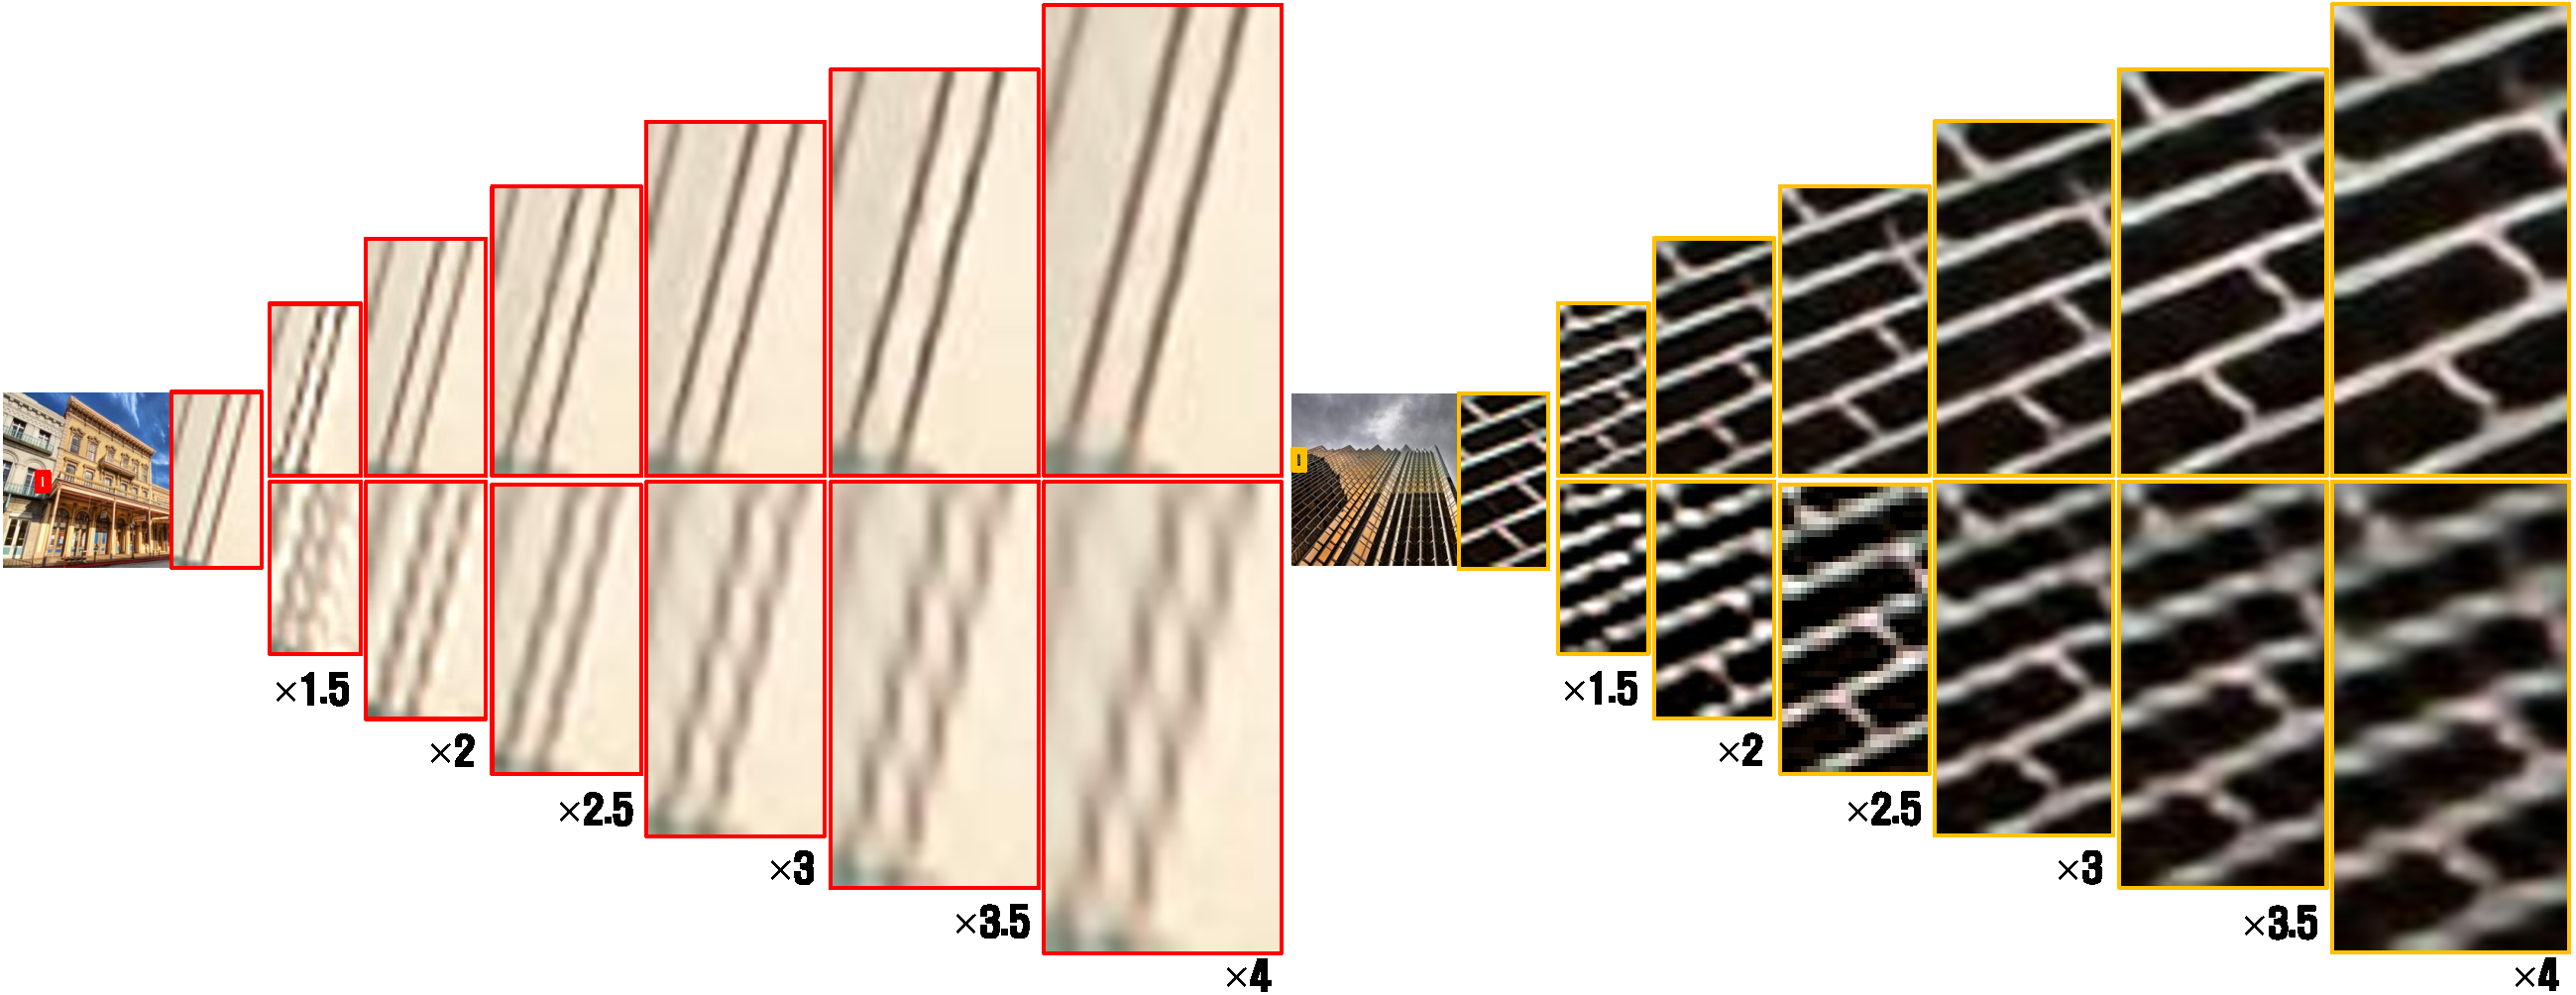
\includegraphics[width=\textwidth]{figs/fig1_sffsr.pdf}
%\end{tabular}
%%\begin{figure*}
%%\includegraphics{figs/sr10.png}
%%\end{figure*}
%}
%\bigskip}% ... an image
%\vspace{-15pt}
%\captionof{figure}{\label{fig:fig1}
%(Top) Our results using a single network for all scale factors. Super-resolved images over all scales are clean and sharp. (Bottom)  Results of Dong et al.  \cite{Dong2014} ($\times$3 model used for all scales). Result images are not visually pleasing. To handle multiple scales, existing methods require multiple networks. }
%\vspace{15pt}
%}
%\makeatother


%%%%%%%%% TITLE
\title{Fast and Accurate Image Super-Resolution Using Very Deep Convolutional Networks}

\author{First Author\\
	Institution1\\
	Institution1 address\\
	{\tt\small firstauthor@i1.org}
	% For a paper whose authors are all at the same institution,
	% omit the following lines up until the closing ``}''.
	% Additional authors and addresses can be added with ``\and'',
	% just like the second author.
	% To save space, use either the email address or home page, not both
	\and
	Second Author\\
	Institution2\\
	First line of institution2 address\\
	{\tt\small secondauthor@i2.org}
}

\maketitle
%\thispagestyle{empty}


%%%%%%%%% ABSTRACT
\begin{abstract}
We present a very fast and accurate single-image super-resolution (SR) method. Our method uses a very deep convolutional network inspired by VGG-net used for ImageNet classification \cite{simonyan2015very}. We find increasing network depth with very small ($3\times 3$) convolution filters show a significant improvement. Our final model uses 20 weight layers. By cascading small filters many times in a deep network structure, contextual information over large image regions is successfully exploited. With very deep networks, however, convergence becomes a critical issue in training. We estimate the residual images instead of high-resolution images. As residuals are sparse, we find the network converges much faster with better accuracy during training. Our proposed method outperforms existing methods by a large margin while very fast.
\end{abstract}

%%%%%%%%% BODY TEXT
\section{Introduction}
We address the problem of generating a high-resolution (HR) image given a low-resolution (LR) image, commonly referred as single image super-resolution (SISR) \cite{Irani1991}, \cite{freeman2000learning}, \cite{glasner2009super}. SISR is widely used in computer vision applications ranging from security and surveillance imaging to medical imaging where more image details are required on demand.

Many SISR methods have been studied in the computer vision community. Interpolation methods such as bicubic interpolation and Lanczos resampling \cite{duchon1979lanczos} are simple and very fast but they give poor results. More powerful methods utilize statistical image priors \cite{sun2008image,Kim2010} or rely on internal patch recurrence \cite{glasner2009super}.

Recently, sophisticated learning methods are widely used to model a mapping from LR to HR patches. Existing methods use various techniques: neighbor embedding \cite{chang2004super,bevilacqua2012}, sparse coding \cite{yang2010image,zeyde2012single,Timofte2013,Timofte} and convolutional neural network (CNN) \cite{Dong2014}.

Among them, Dong et al. \cite{Dong2014} has demonstrated that a CNN can be used to learn a mapping from LR to HR in an end-to-end manner. Their method, termed SRCNN, does not require any engineered features that are typically necessary in other methods \cite{yang2010image,zeyde2012single,Timofte2013,Timofte}. In addition, it is very fast and accurate.

While SRCNN successfully introduced a deep learning technique into the super-resolution (SR) problem, we find its limitations in three aspects: first, it relies on context of small image regions; second, training converges slowly; third, the network only works for single-scale.

In this work, we propose a new method to practically resolve the issues.


\textbf{Context} We utilize contextual information spread over very large image regions. For a large scale factor, it is often the case that information contained in a small patch is not sufficient for detail recovery (ill-posed). Our very deep network using large receptive field is aware of large context necessary for large-scale super-resolution.

\textbf{Convergence} We suggest a way to speed-up the training: residual-learning CNN. As LR image and HR image share the same information to a large extent, explicitly modelling the residual image which is the difference between HR and LR images is advantageous. We propose a network structure for efficient learning when input and output are highly correlated.

\textbf{Scale Factor} We propose a single-model SR approach. Scales are typically user-specified and can be arbitrary including fractions. For example, one might need smooth zoom-in in an image viewer or resizing to a specific dimension. Training and storing many scale-dependent models in preparation for all possible scenarios is impractical. We find a single convolutional network is sufficient for multi-scale-factor super-resolution.


\textbf{Contributions} In summary, in this work, we propose a very practical SR method: fast and accurate. Our method based on a very deep convolutional network can be used to super-resolve an image very clean and sharp. Our algorithm demonstrates the state-of-the-art quality for all benchmarked datasets.

%Learning a mapping between low/high-resolution (LR/HR) images
%Many single image super-resolution (SR) methods are based on learning a mapping
%Transferring among scale factors???
%Writing direction: show data augmentation works for some methods.
%show limitation of SRCNN and possibly other methods.
%needs bigger depth for higher scale factors. big depth can be handled by residual-learning, faster convergence and blah.

\section{Related Work}
\begin{figure*}[t]
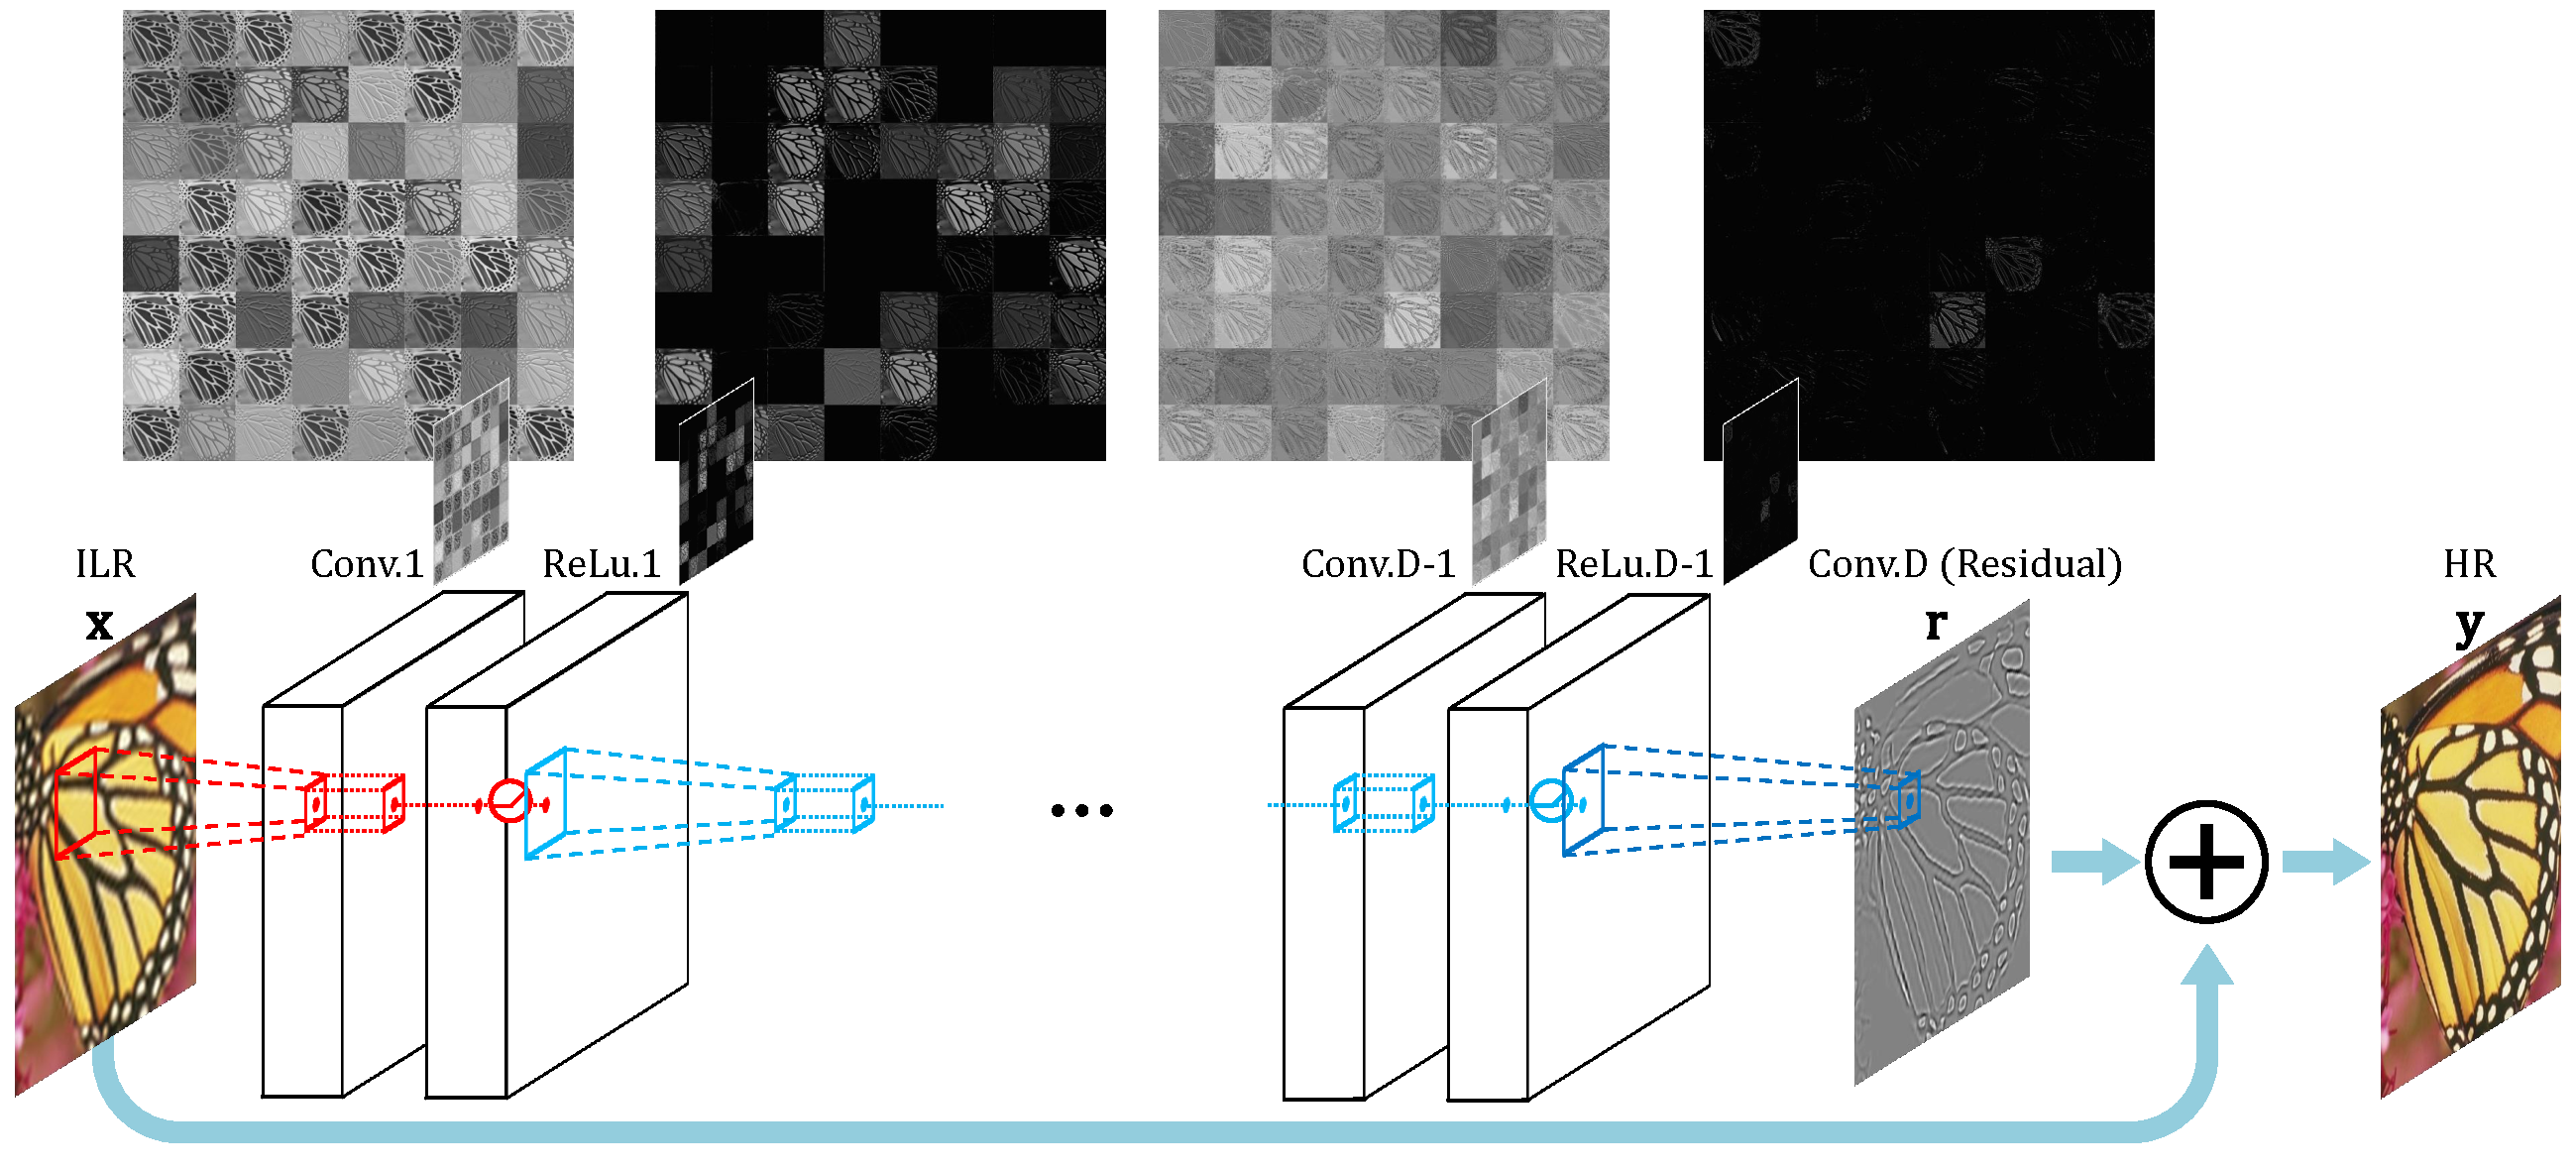
\includegraphics[width=\textwidth]{figs/fig2_sffsr.pdf}
\caption{Our Network Structure. We cascade a pair of layers (convolutional and nonlinear) repeatedly. An interpolated low-resolution image (ILR) go through layers and transforms into a high-resolution image (HR). The network predicts a residual image and addition of ILR and residual gives the desired output. We use 64 filters for each convolutional layer and some sample feature maps are drawn for visualization. Most features after applying rectified linear units (ReLu) are zero.}
\label{fig:network}
\end{figure*}

\subsection{Convolutional Network for Image Super-Resolution}
Recently, Dong et al. \cite{dong2015image} have presented a SR method called SRCNN using a convolutional network. Let us first analyze SRCNN in three aspects: context, convergence and scale.

\textbf{Context}
SRCNN consists of only three layers: patch extraction/representation, non-linear mapping and reconstruction. They use filters with varying spatial sizes $9\times9$, $1\times1$, $5\times5$, respectively. In \cite{dong2015image}, they conclude that deeper networks do not result in better performance in Figure 9.

But we argue that increasing depth significantly boosts the performance. Their experiments failed to show the gain from deeper structure because their deeper versions converged very slowly and they early stopped the training.

In contrast, we successfully use 20 weight layers($3\times3$ for each layer). Our network is very deep (20 vs. 3\cite{dong2015image}) and information used for reconstruction (receptive field) is much larger ($41\times41$ vs. $13\times13$\cite{dong2015image}).

\textbf{Convergence}
For training, SRCNN directly model high-resolution images so that the convergence rate is very slow. In contrast, our network models the residual images, i.e., the image details. We find convolution network converge much faster with better accuracy during training.

\textbf{Scale} SRCNN is trained for a single scale factor and supposed to work only with the specified scale. Given a user-specified scale, the corresponding network is retrieved for the task. If new scale is on demand, new model has to be trained. Most existing methods including not only SRCNN but also other regression-based methods \cite{Timofte2013, Timofte, Yang2013} are in this paradigm. So, in these frameworks, the general super-resolution task is decomposed into multiple sub-tasks, where each sub-task is a single-scale super-resolution. Each sub-task is solved by a super-resolution machine, trained to be an expert for the corresponding scale. 

However, preparing many individual machines for all possible scenarios to cope with multiple scales is inefficient since many systems with the same structure need to be trained and stored.
We attempt to reinterpret the task in our work and try to use a single machine to solve all sub-tasks, multi-scale. This turns out to work very well. Our single machine is compared favorably to a single-scale expert for the given sub-task. For three scales factors ($\times 2,3,4$), we can reduce the number of parameters three-fold.


With above improvements, our network delivers a great performance. In addition, our output image has the same size as the input image by padding zeros every layer during training whereas output from SRCNN is smaller than the input. Finally, we simply use the same learning rates for all layers while SRCNN uses different learning rates for different layers.

\begin{table*}[t]
	\small
	\centering
\begin{tabular}
{|c|c|c|c|c|c|c|c||c|}
\hline 
 Test / Train & {$\times$2}& {$\times$3}& { $\times$4}& {$\times$2,3}& {$\times$2,4}& { $\times$3,4}& {$\times$2,3,4} & {Bicubic} \\
\hline
$\times$2  & \color{red} 37.10  & 30.05  & 28.13  & \color{red} 37.09  & \color{red} 37.03  & 32.43  & \color{red}37.06 &33.66   \\
$\times$3  & 30.42  & \color{red} 32.89  & 30.50  & \color{red} 33.22  & 31.20  & \color{red} 33.24  & \color{red} 33.27  & 30.39 \\
$\times$4  & 28.43  & 28.73  & \color{red} 30.84  & 28.70  & \color{red} 30.86  & \color{red} 30.94  & \color{red} 30.95 & 28.42  \\
\hline
\end{tabular}
	\vspace{1pt}
	\caption{Scale Factor Experiment. Several models are trained with different scale sets. Quantitative evaluation (PSNR) on dataset `Set5' is provided for scale factors 2,3 and 4.  {\color{red}Red color} indicates test scale is included during training. Models trained with multiple scales perform well on the trained scales. }
	\label{tab:SRCNN_Factor_Test}
\end{table*}

\section{Proposed Method}
In this section, our proposed method is explained in detail. We first go over the process of super-resolving an image with a convolutional neural network (inference). Next, we visit the training procedure for a convolutional network.
\subsection{Inference}

For reconstruction, we use a very deep convolutional network inspired by Simonyan and Zisserman \cite{simonyan2015very}. The configuration is outlined in Figure \ref{fig:network}. We use $d$ layers where layers except the first and the last are of the same type: 64 filter of the size $3\times 3 \times64$, where a filter operates on $3\times3$ spatial region across 64 channels (feature maps). The first layer operates on the input image. The last layer, used for image reconstruction, consists of a single filter of size $3\times 3 \times64$.

The network takes an interpolated input image (to the desired size) as input and predicts image details. While modelling image details is often used in super-resolution methods \cite{Timofte2013, Timofte, bevilacqua2012,bevilacqua2013super}, to our knowledge, there has been no CNN-based method that models image details explicitly.

In this work, we demonstrate explicitly modelling image details is sufficient for the purpose of SR and has several advantages. These are further justified and discussed later in the Section \ref{sec:residual}. 

One problem with applying a deep network to predict dense outputs is that the size of feature map gets reduced every time convolution operations are applied. For example,  when an input of size $(n+1)\times (n+1)$ is applied to a network with receptive field size $n\times n$, the output image is $1\times1$. 

This is in accordance with other super-resolution methods since many require surrounding pixels to infer center pixels correctly. This center-surround relation is useful since surrounding region provides more constraints to this ill-posed problem (SR). For pixels near image boundary, this relation cannot be exploited to the full extent and many SR methods crop the result image. 

This methodology, however, is not valid if required surround region is very big. After cropping, the final image is too small to be visually pleasing.

To resolve this issue, we opt not to use this relation. Instead, we use the same-sized regions (i.e. $n\times n$ input and output). To do this, we pad zeros before convolutions to keep the sizes of all feature maps (including the output image) the same. We think that powerful nonlinearities modelled by CNNs can handle both the general case (i.e. receptive field has all valid pixels) and the corner case (i.e. the field located near the image boundary has invalid pixels beyond the border).

It turns out that zero-padding works surprisingly well. For this reason our method differs from most other methods in the sense that pixels near image boundary are also correctly predicted. 

Once image details are predicted, they are added back to ILR to give the final result (HR). We use this structure for all experiments in our work.  




\begin{figure*}[t]
	\centering
	\begin{subfigure}{0.3\textwidth}
		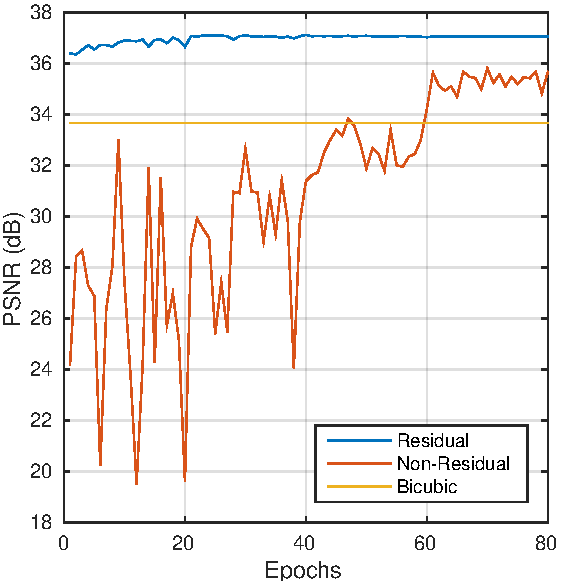
\includegraphics[width=\textwidth]{figs/residual_exp0}
		\caption{Initial learning rate 0.1}
		\label{fig:gull}
	\end{subfigure}%
	\hfill
	%(or a blank line to force the subfigure onto a new line)
	\begin{subfigure}{0.3\textwidth}
		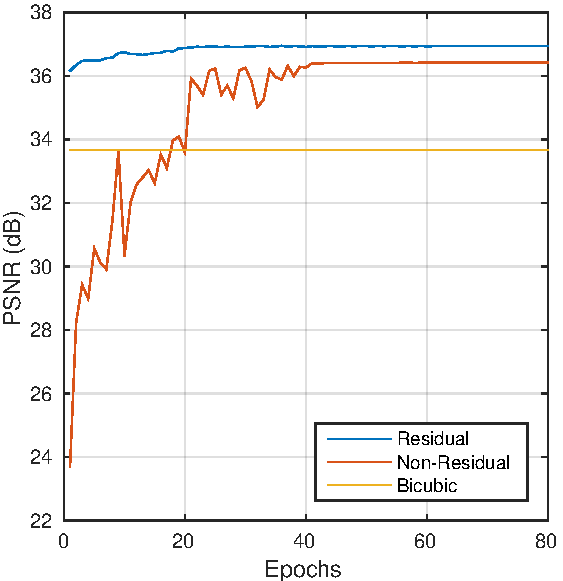
\includegraphics[width=\textwidth]{figs/residual_exp1}
		\caption{Initial learning rate 0.01}
		\label{fig:tiger}
	\end{subfigure}
	\hfill
	\begin{subfigure}{0.3\textwidth}
		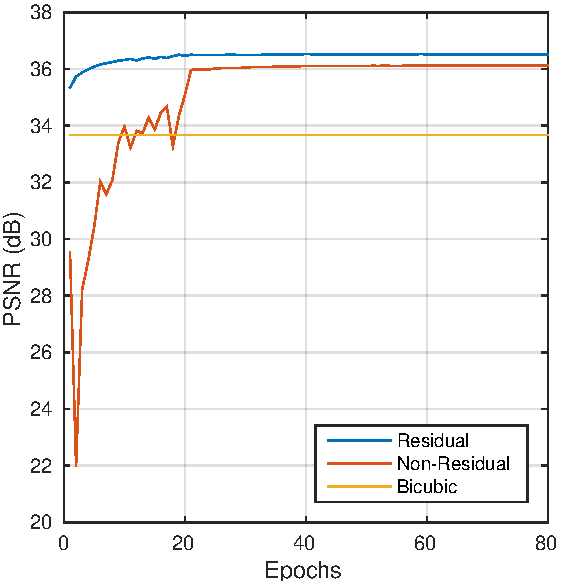
\includegraphics[width=\textwidth]{figs/residual_exp2}
		\caption{Initial learning rate 0.001}
		\label{fig:mouse}
	\end{subfigure}
	\caption{Performance curve for residual and non-residual networks. Two networks are tested under `Set5' dataset with scale factor 2. Residual networks quickly reaches state-of-the-art performance within a few epochs, whereas non-residual network (which models high-resolution image directly) takes many epochs to reach its maximum performance. Moreover, the final accuracy is higher for residual network.}
	\label{fig:residual2}
\end{figure*}

\begin{figure*}
\centering
\begin{subfigure}{0.3\textwidth}
\centering
{\graphicspath{{figs/graph1/}}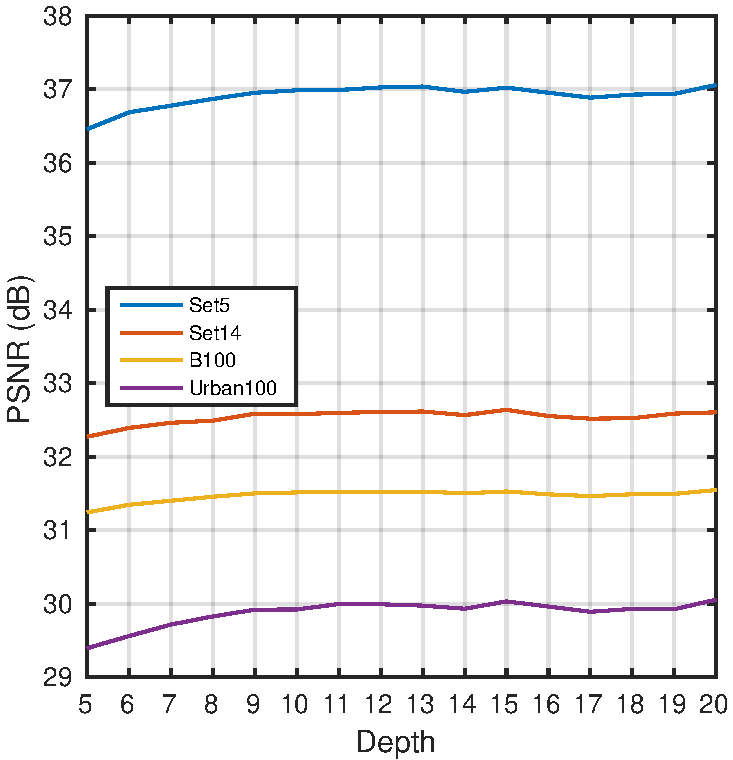
\includegraphics[height=4.8cm]{graph2.pdf}}
\caption{Test Scale Factor 2}
\end{subfigure}%
\begin{subfigure}{0.3\textwidth}
\centering
{\graphicspath{{figs/graph1/}}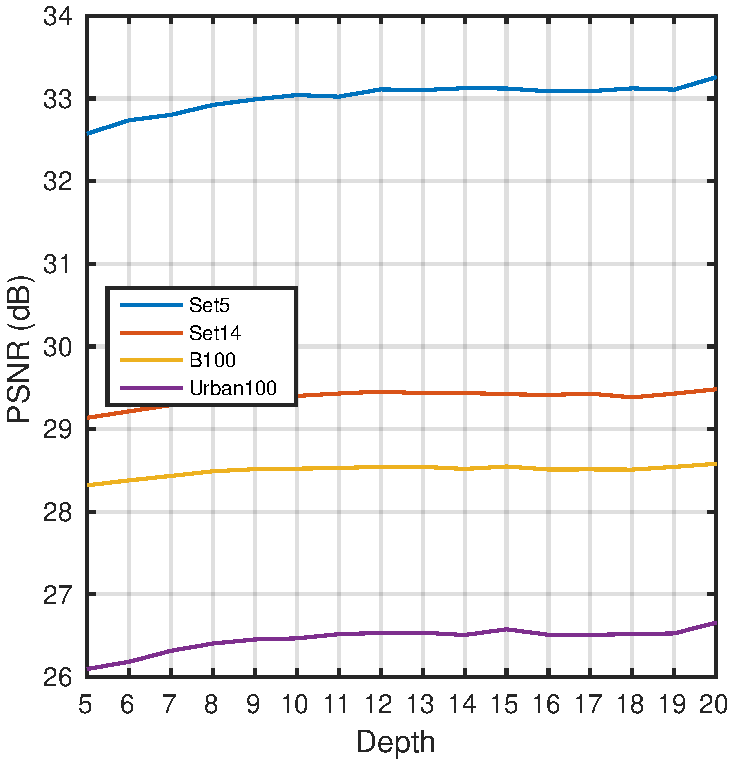
\includegraphics[height=4.8cm]{graph3.pdf}}
\caption{Test Scale Factor 3}
\end{subfigure}%
\begin{subfigure}{0.3\textwidth}
\centering
{\graphicspath{{figs/graph1/}}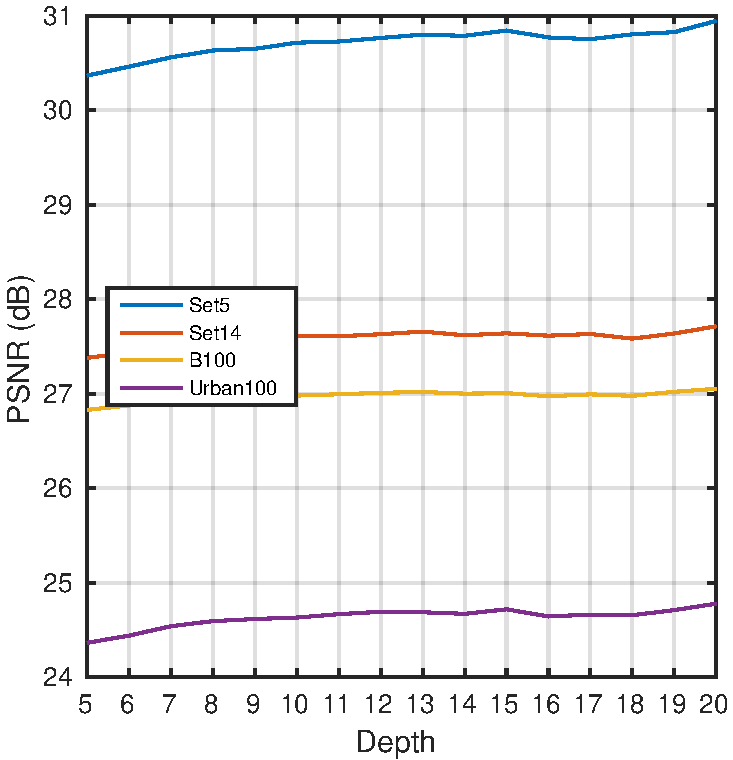
\includegraphics[height=4.8cm]{graph4.pdf}}
\caption{Test Scale Factor 4}
\end{subfigure}%
\caption{Depth vs Performance}
\end{figure*}


\subsection{Training}

We now describe the objective to minimize to find optimal parameters of our model. Let ${\bf x}$ denote an interpolated low-resolution image and ${\bf y}$ a high-resolution image. 
Given training dataset $\{{\bf x}^{(i)},{\bf y}^{(i)}\}{}_{i=1}^{N}$, our goal is to learn a model $f$ that predicts values $\mathbf{\hat{y}}=f(\mathbf{x})$.

In the least-squares regression setting, typically used in super-resolution
problems, the mean squared error $\frac{1}{2}||\mathbf{y}-f(\mathbf{x})||^{2}$
averaged over training set is minimized. This favors high Peak Signal-to-Noise
Ratio (PSNR), a widely-used evaluation criteria for SR. 

As the input and output images are mostly similar, we define a residual image ${\bf r}={\bf y}-{\bf x}$, where most values are likely to be zero or small. We want to predict this residual image. The loss function now becomes $\frac{1}{2}||\mathbf{r}-f(\mathbf{x})||^{2}$, where $f(\bf{x})$ is the network prediction. Loss function is one major difference between SRCNN and ours. 

In networks, this is reflected in the loss layer as follows. 
Our loss layer takes three inputs: residual estimate, network input (ILR) and ground truth HR. The loss is computed as the Euclidean distance between the reconstructed image (the sum of network input and output) and ground truth. With this residual loss layer, we can still use the original dataset for an end-to-end learning.

Training is carried out by optimizing the regression objective using mini-batch gradient descent based on back-propagation (LeCun et al. \cite{lecun1998gradient}). We set the momentum parameter to 0.9. The training is regularized by weight decay ($L_2$ penalty multiplied by
0.0001).  

Training deep models often fail to converge. He et al. \cite{he2015delving} uses a theoretically sound initialization method which helps very deep models converge when training from scratch and they succeed in training 30 weight layers. They, however, report no benefit from training extremely deep models for their problem. In our work, adding layers are beneficial in general. For large scale factors, deep models exploiting contextual information spread in very large field are dominant. 

Training the multi-scale model is straightforward. Training datasets for several specified scales are combined into one big dataset. We demonstrate in the next section that a model learned with this works under multiple scales.  

Data preparation is similar to SRCNN \cite{Dong2014} with some differences. Input patch size is equal to the size of receptive field and images are divided into sub-images with no overlap. 64 sub-images constitue a mini-batch, where sub-images from different scales can be in the same batch.

We implement our model using the \textit{MatConvNet}\footnote{\url{ http://www.vlfeat.org/matconvnet/}} package \cite{arXiv:1412.4564}.

\section{Understanding Properties}

In this section, we study three properties of our proposed method. First, we show our method with a single network performs as well as a method using multiple networks trained for each scale. We can effectively reduce model capacity (the number of parameters) of multi-network approaches.

Second, we show our residual-learning network converges very fast in relative to the standard CNN. Moreover, our network gives a significant boost in performance. 

Third, we show large depth is necessary for the task of SR. A very deep network utilizes more contextual information in an image and models complex functions with many nonlinear layers. We experimentally confirm that deeper networks give better performances than shallow ones. 

\subsection{Single Model for Multiple Scales}
Scale augmentation during training is a key technique to equip a network with super-resolution machines of multiple scales. Many SR processes for different scales can be executed with our multi-scale machine with much smaller capacity than that of single-scale machines combined. 

We start with an interesting experiment as follows: we train our network with a scale factor $s_{\text{train}}$ and it is tested under another scale factor $s_{\text{test}}$. Here, factors 2,3 and 4 that are widely used in SR comparisons are considered. Possible pairs ($s_{\text{train}}$,$s_{\text{test}}$) are tried for the dataset `Set5' \cite{bevilacqua2012}. Experimental results are summarized in Table \ref{tab:SRCNN_Factor_Test}. 

Performance is degraded if $s_{\text{train}} \neq s_{\text{test}}$. For scale factor 2, the model trained with factor 2 gives PSNR of 37.10 (in dB), whereas models trained with factor 3 and 4 give 30.05 and 28.13, respectively. A network trained over single-scale data is not capable of handling other scales. In many tests, it is even worse than bicubic interpolation, the method used for generating the input image. 

We now test if a model trained with scale augmentation is capable of performing SR at multiple scale factors. The same network used above is trained with multiple scale factors $s_{\text{train}} = \{2,3,4\}$. In addition, we experiment with the cases $s_{\text{train}} = \{2,3\}, \{2,4\}, \{3,4\}$ for more comparisons. 

We observe the network copes with any scale used during training. When $s_{\text{train}} = \{2,3,4\}$ ($\times 2, 3, 4$ in Table \ref{tab:SRCNN_Factor_Test}), its PSNR for each scale is comparable to those achieved from the corresponding result of single-scale network: 37.06 vs. 37.10 ($\times 2$), 33.27 vs. 32.89 ($\times 3$), 30.95 vs. 30.86 ($\times 4$).

Another pattern is that for large scales ($\times 3,4$), our multi-scale network performs over single-scale network: our model ($\times 2,3$), ($\times 3,4$) and ($\times 2, 3,4$) give PSNRs 33.22, 33.24 and 33.27 for test scale 3, respectively, whereas ($\times 3$) gives 32.89. Similarly, ($\times 2,4$), ($\times 3,4$) and ($\times 2, 3,4$) give 30.86, 30.94 and 30.95 (vs. 30.84 by $\times 4$ model),  respectively. From this, we observe training multiple scales boost the performance for large scales.

\subsection{Residual Images for Better Learning}
\label{sec:residual}

As we already have low-resolution image as input, predicting high-frequency components is enough for the purpose of SR. Predicting residuals (HR - ILR) is widely used in several previous methods \cite{Timofte2013, Timofte,zeyde2012single}. However, it has not been studied in the context of deep-learning-based SR.

In this work, we have proposed a network structure that learns from a residual image (ground truth minus input, i.e. high-resolution image minus interpolated low-resolution). We now study the effect of this modification to a standard CNN structure in detail. 

First, we find this residual network converge much faster. Two networks are compared experimentally: residual network and standard network. We use depth 10 (weight layers) and scale factor 2. Performance curves for various learning rates are shown in Figure \ref{fig:residual2}. All use the same learning rate scheduling mechanism that has been mentioned above. 

Second, at convergence, the residual network shows superior performance. In Figure \ref{fig:residual2}, residual networks give higher PSNR when training is done. 

In short, this simple modification to a standard network structure is beneficial and one can explore the validity of the idea in other image restoration problems. 

\begin{figure}
\vspace{-1cm}
\centering
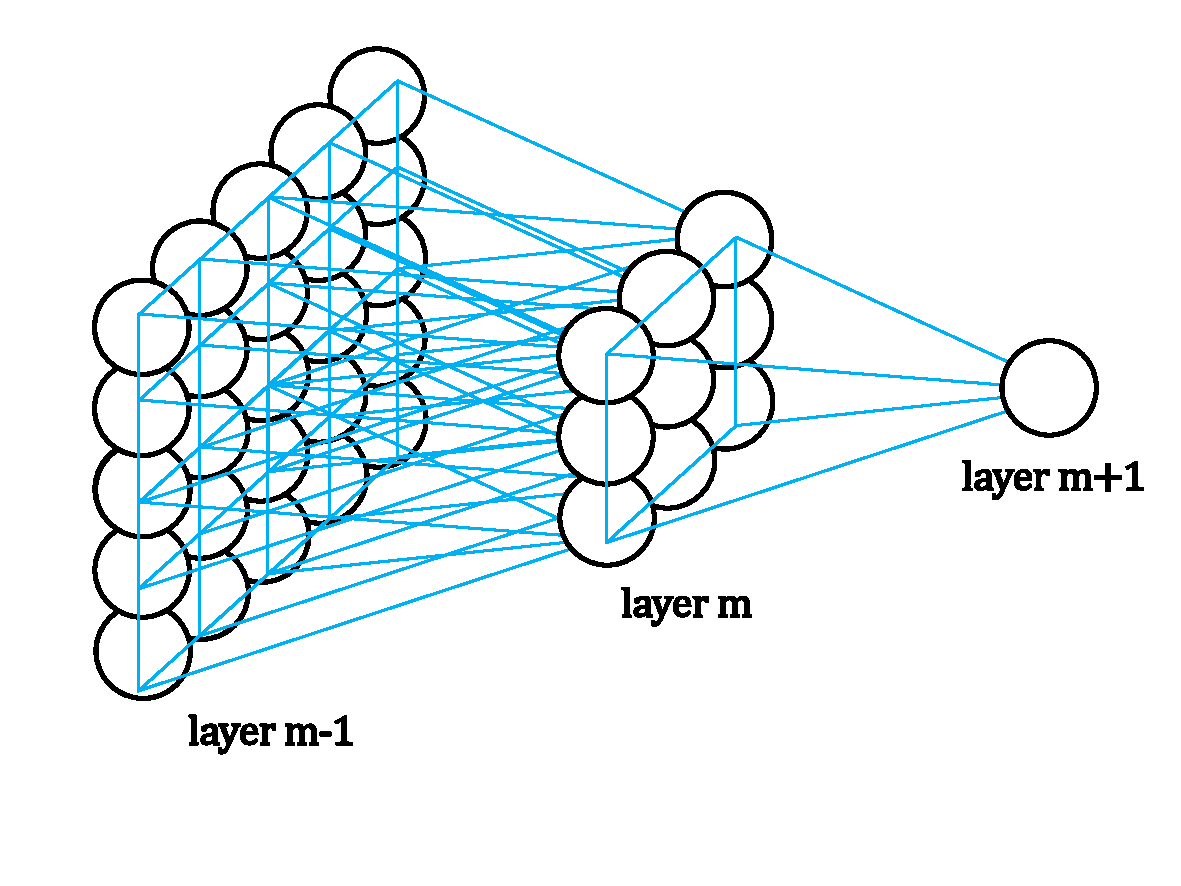
\includegraphics[scale=0.3]{figs/fig4_sffsr.pdf}
\vspace{-0.7cm}
\caption{Receptive field for a neuron in network grows as layers are stacked. In our work, up to 20 layers are used reaching 41$\times$41 at maximum. }
\label{fig:receptive_field}
\end{figure}


\begin{figure*}
\begin{center}
\begin{tabular}{ccccc}
\graphicspath{{figs/}}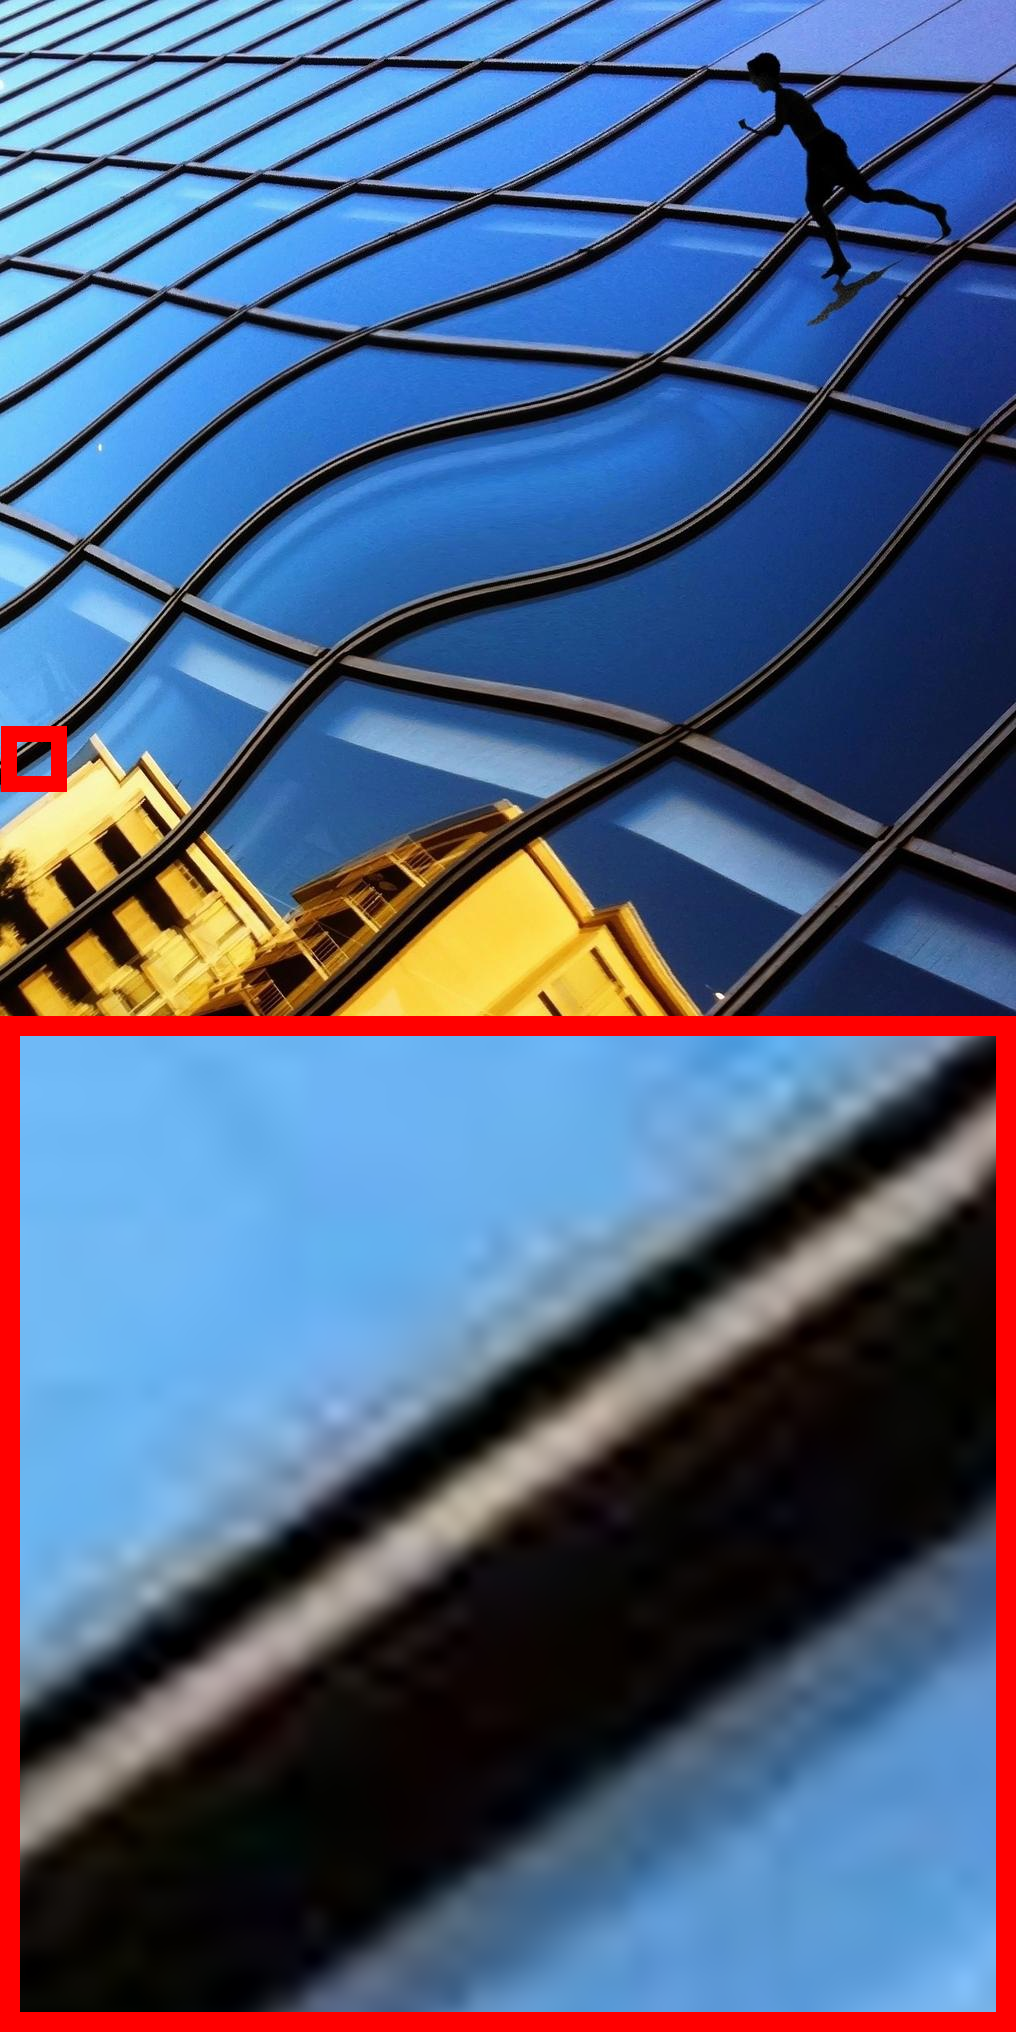
\includegraphics[width=0.18\textwidth]{img_082_1_w.png} &
\graphicspath{{figs/}}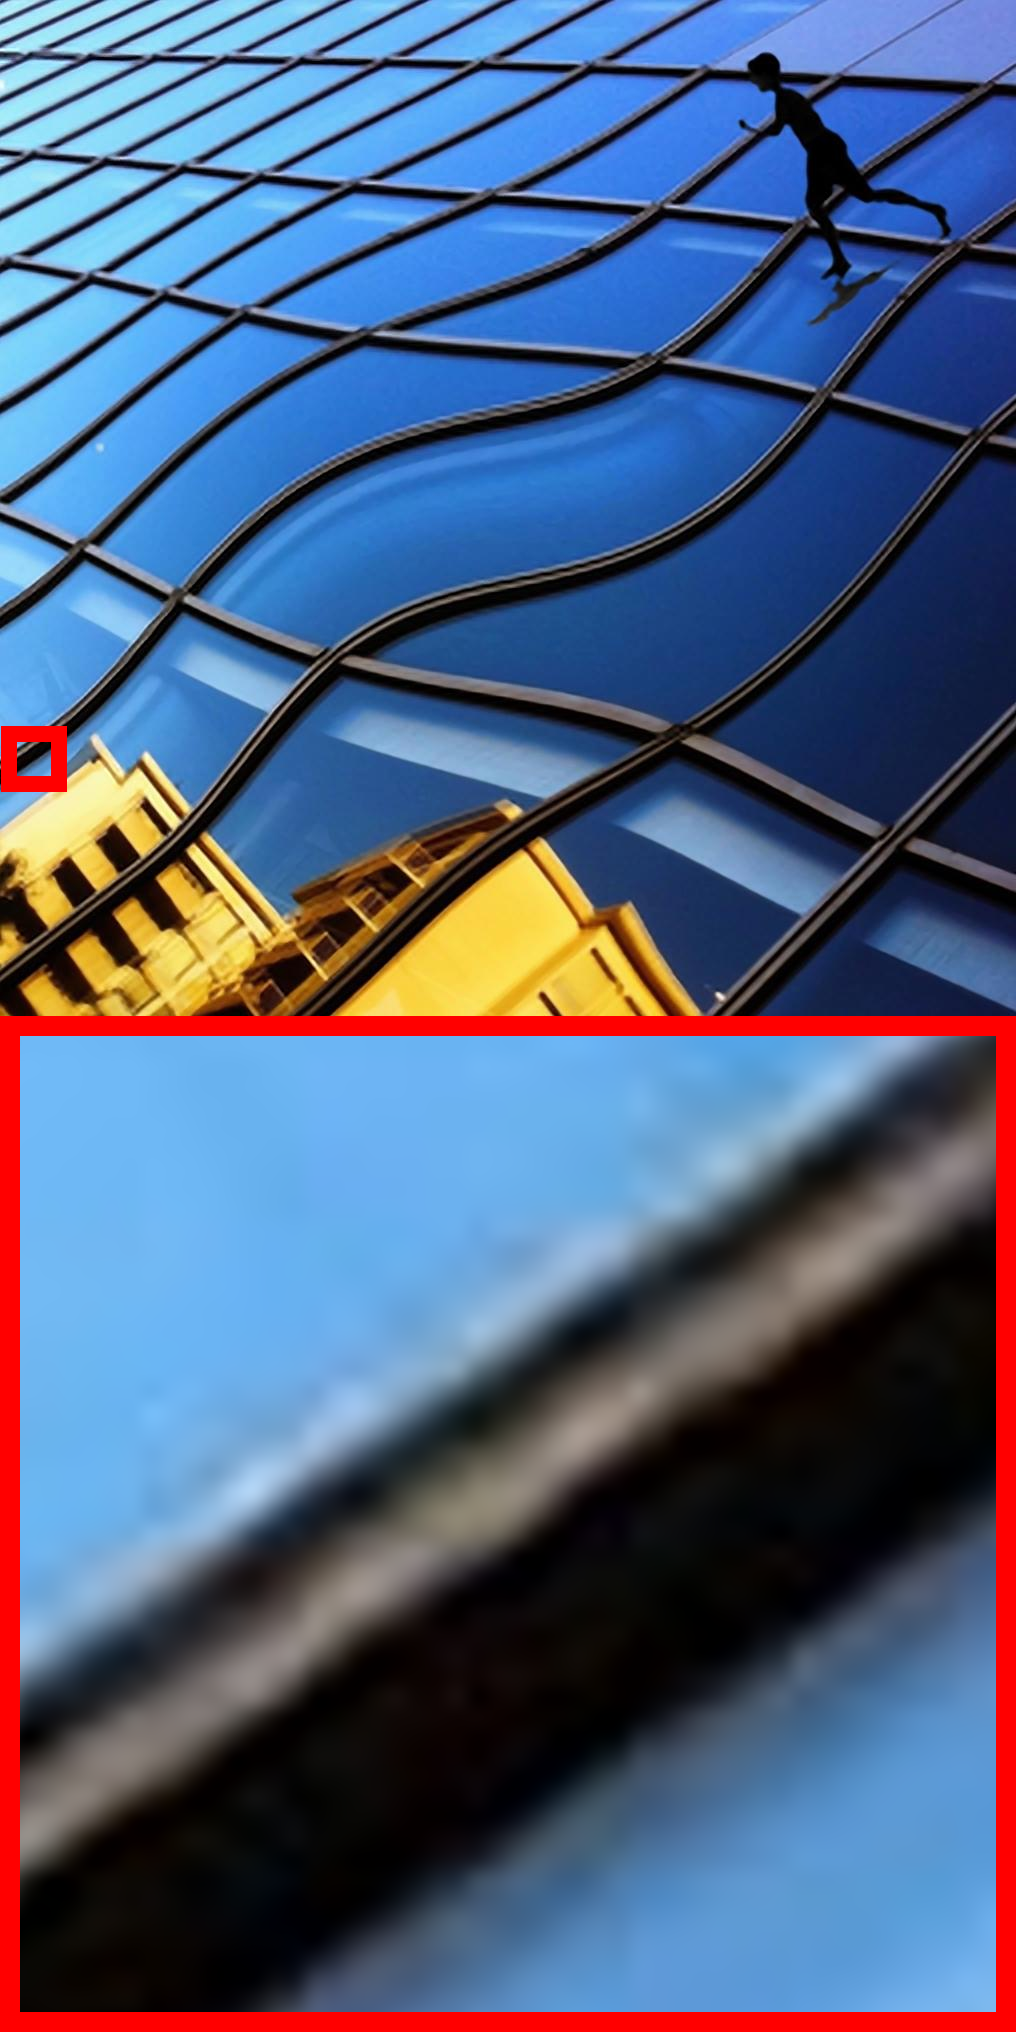
\includegraphics[width=0.18\textwidth]{img_082_6_w.png} &
\graphicspath{{figs/}}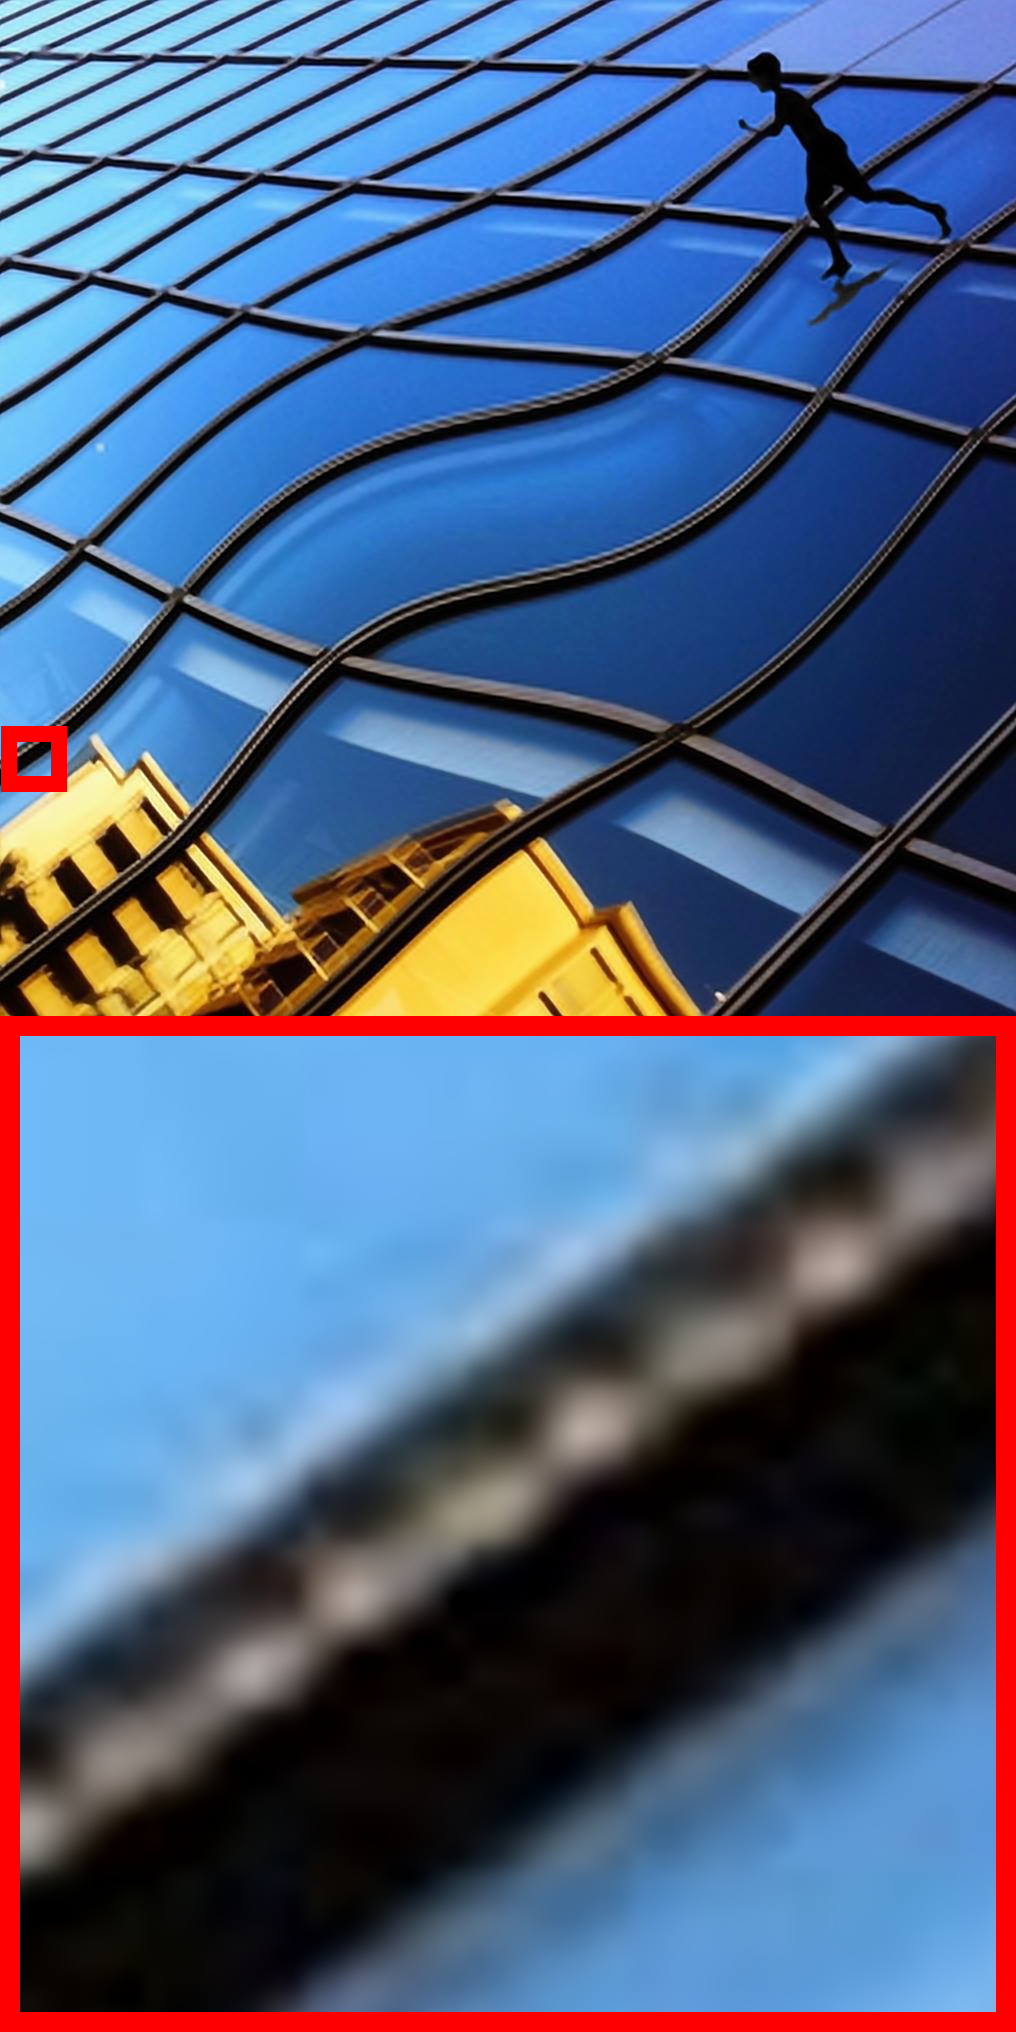
\includegraphics[width=0.18\textwidth]{img_082_7_w.png} &
\graphicspath{{figs/}}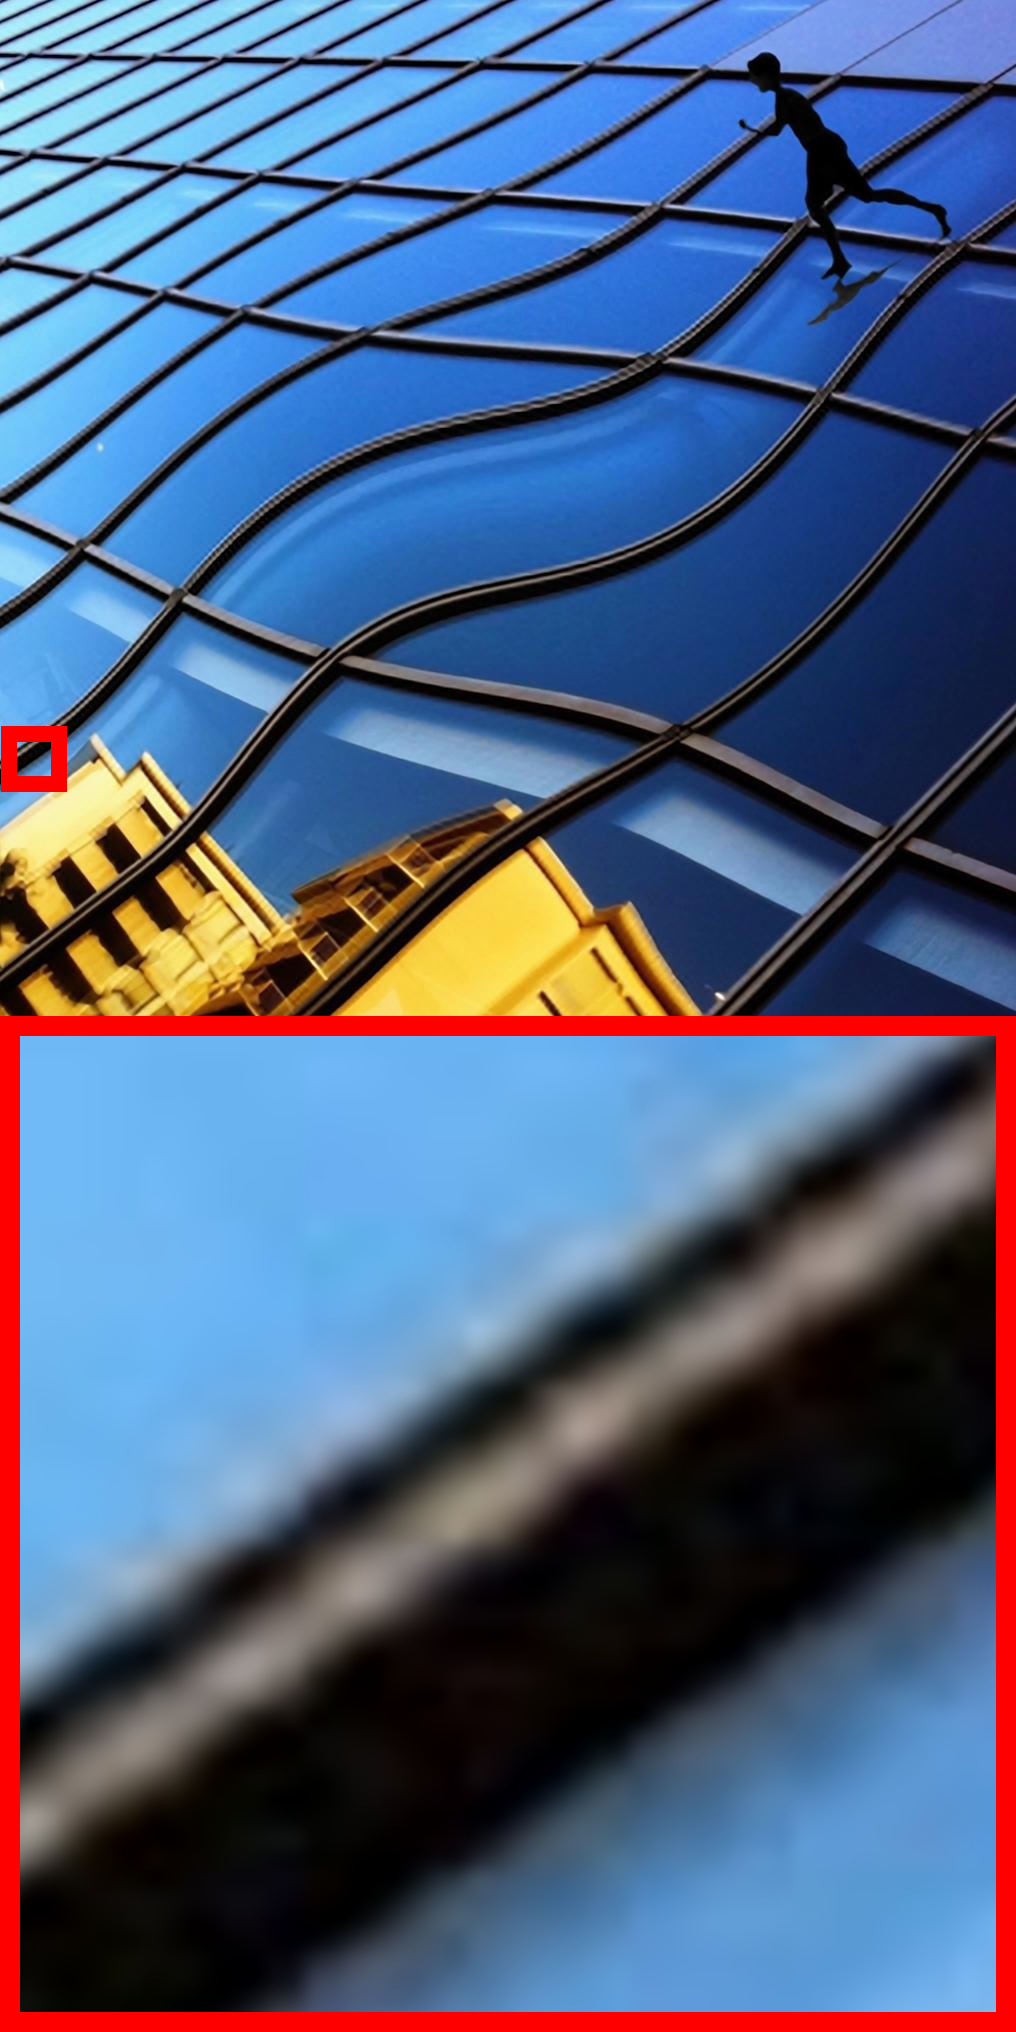
\includegraphics[width=0.18\textwidth]{img_082_10_w.png} &
\graphicspath{{figs/}}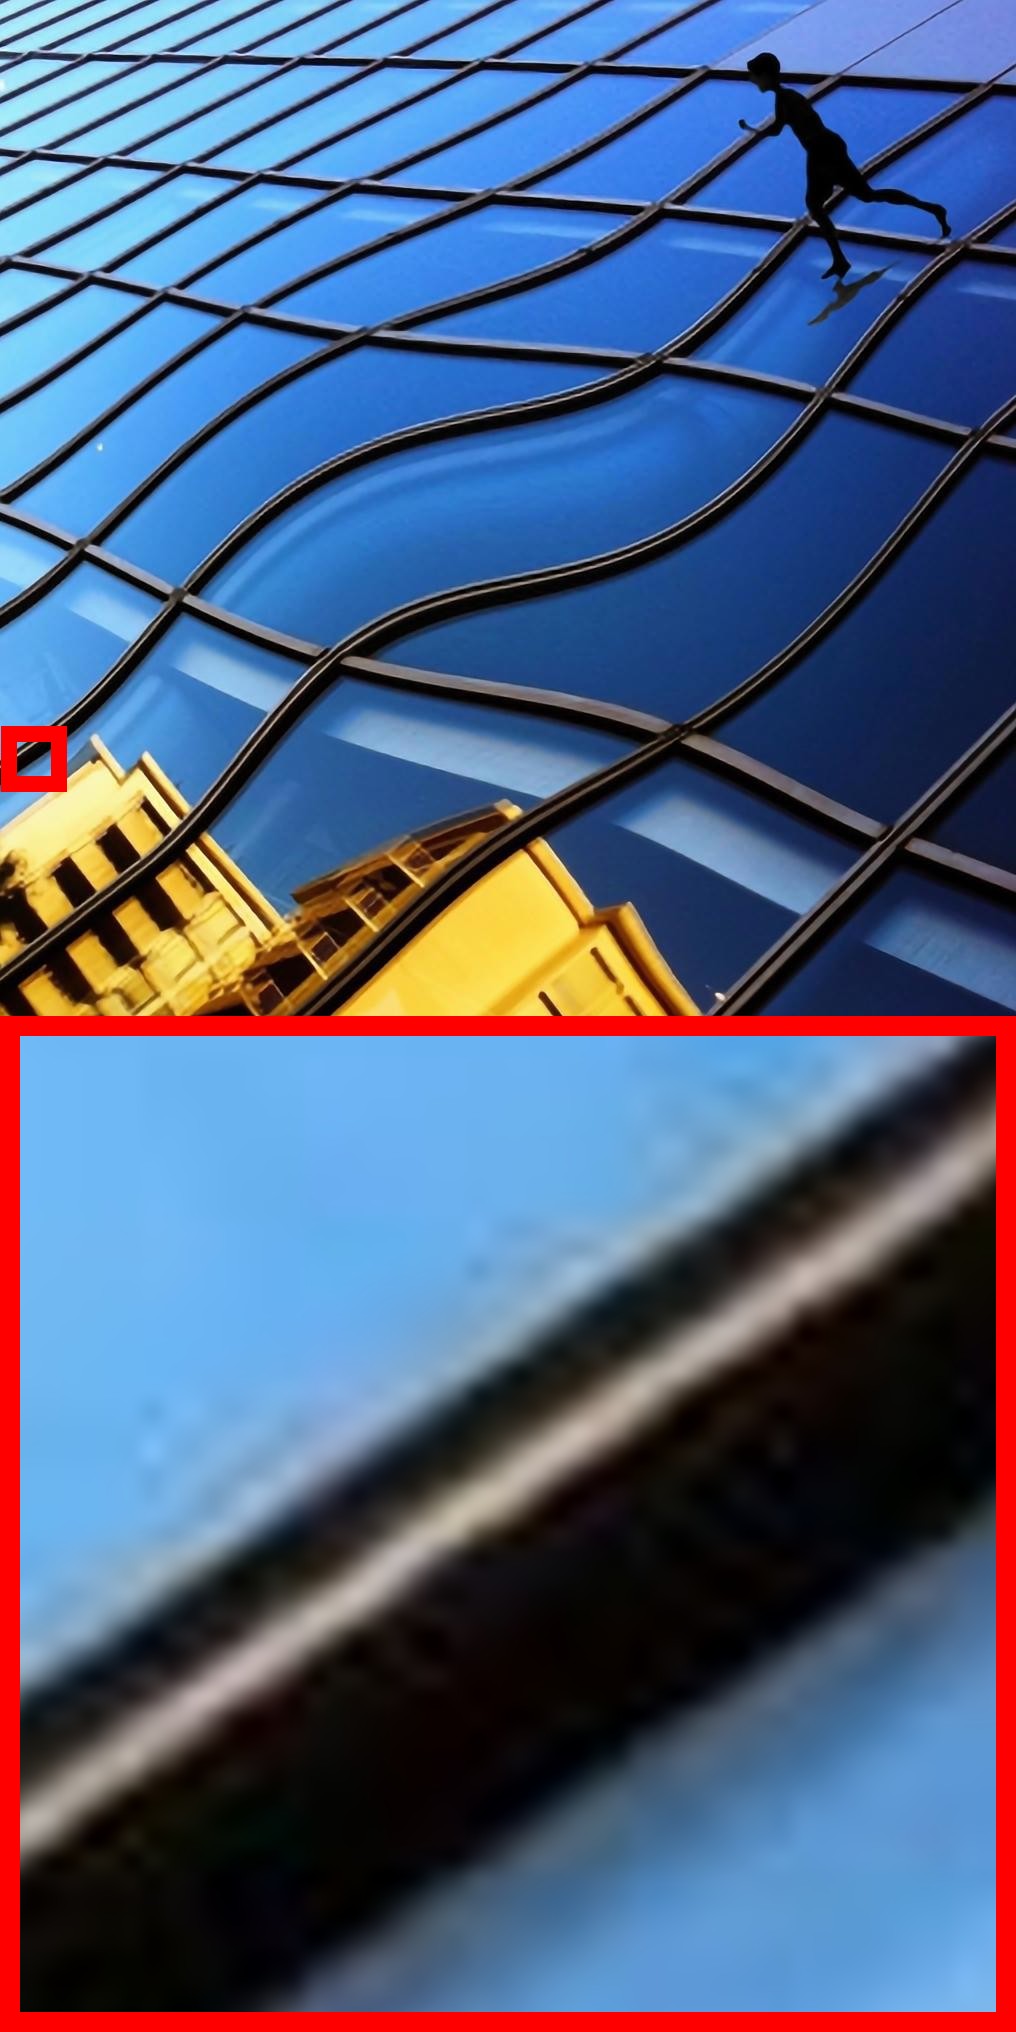
\includegraphics[width=0.18\textwidth]{img_082_9_w.png} 
\\
Original / PSNR (dB) &A+ / 29.84 &SRCNN / 29.20 &Huang et al. / 30.17 &RCN (Ours) / 30.86 \\
\end{tabular}
\end{center}
\vspace{-.5cm}
\caption{Super-resolution results (Urban100) with scale factor $\times$4 Our result is visually pleasing. }\label{fig:c1}
\end{figure*}

\begin{figure*}
\begin{center}
\begin{tabular}{cccc}
\graphicspath{{figs/}}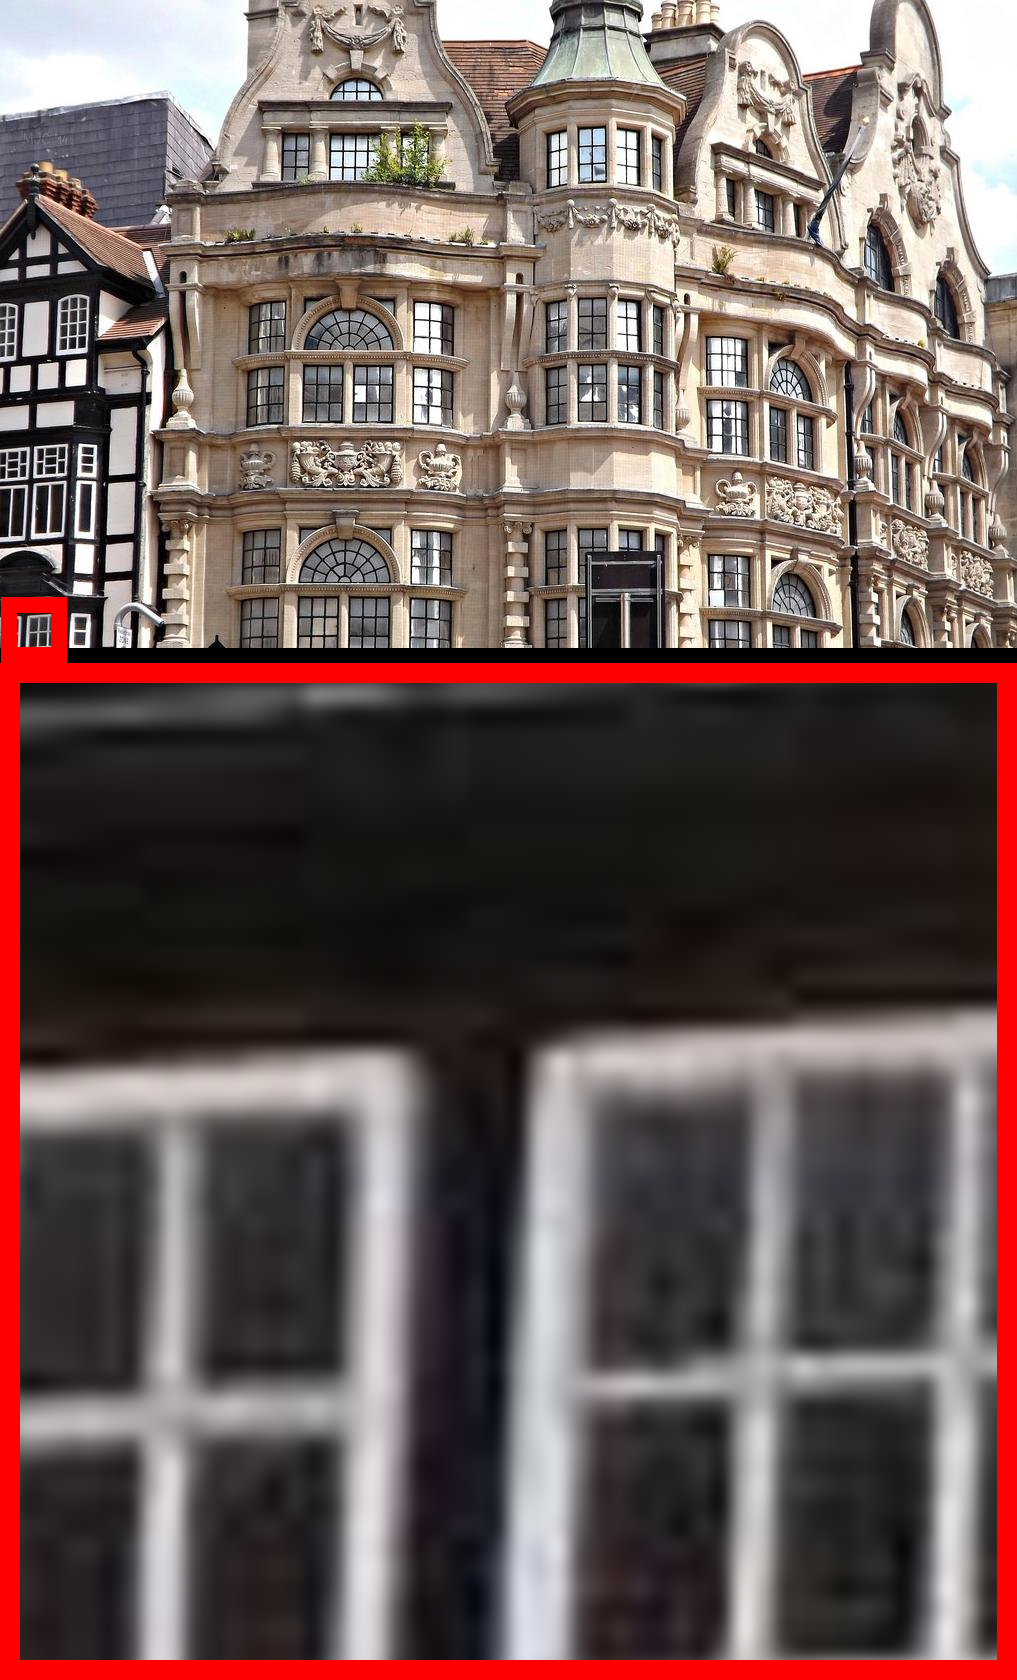
\includegraphics[width=0.23\textwidth]{img_053_1_w.png} &
\graphicspath{{figs/}}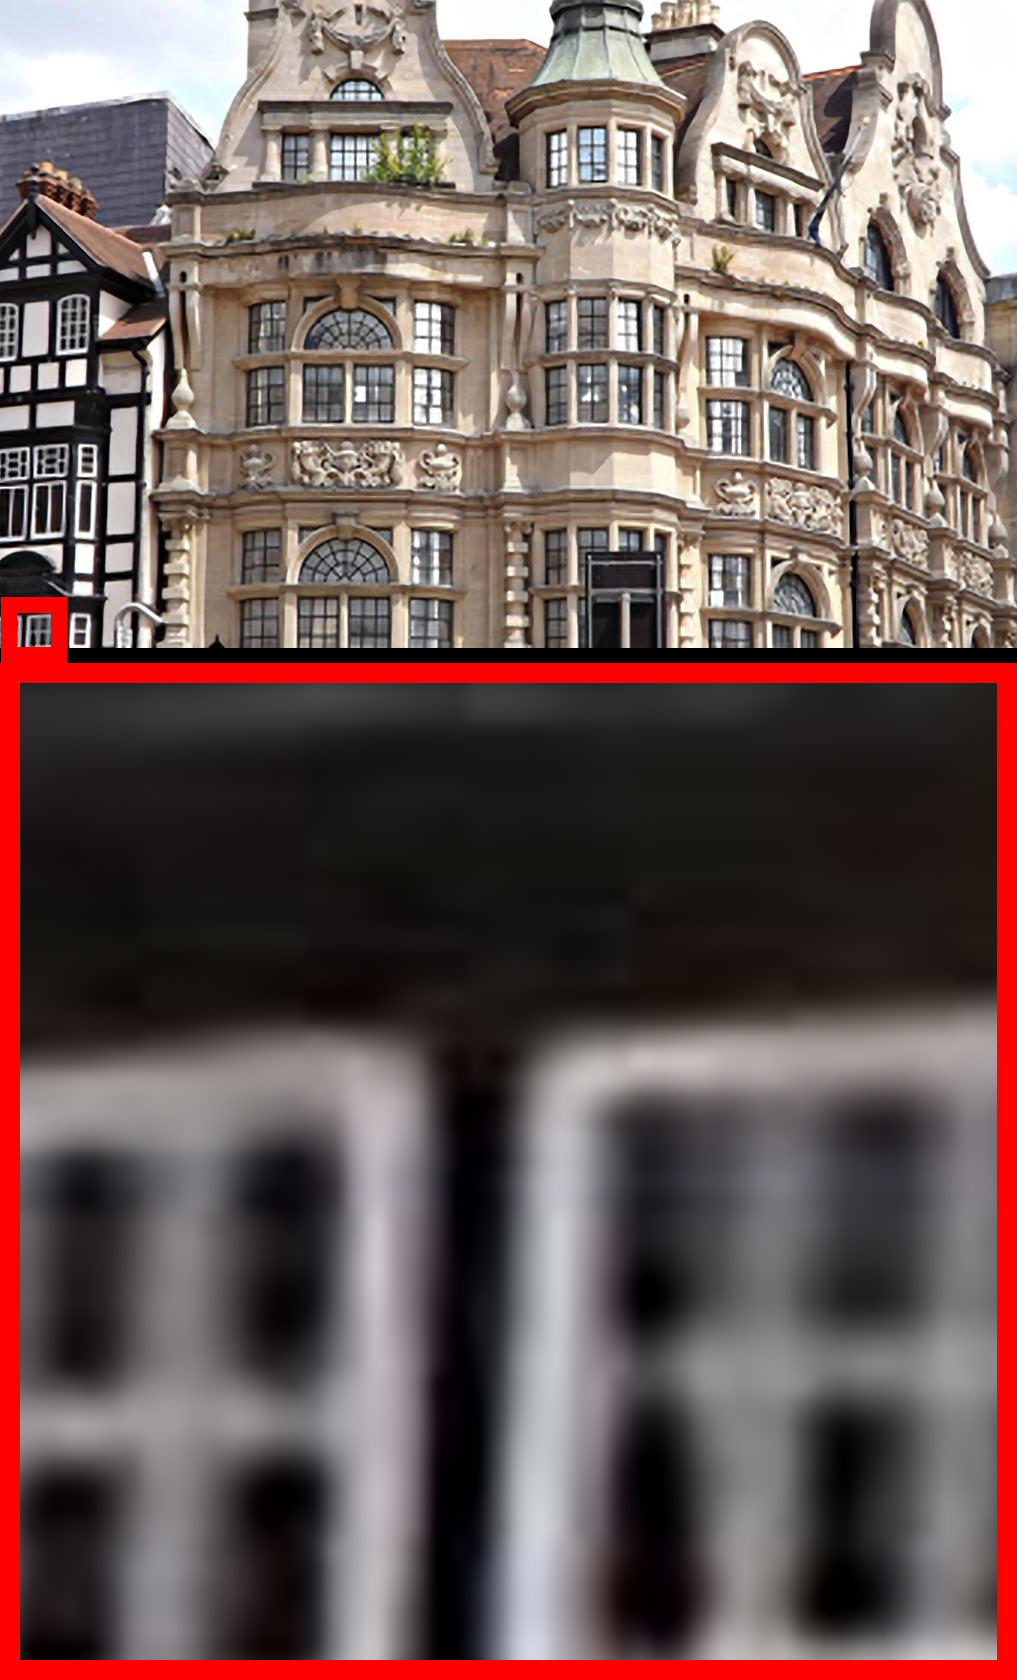
\includegraphics[width=0.23\textwidth]{img_053_6_w.png} &
\graphicspath{{figs/}}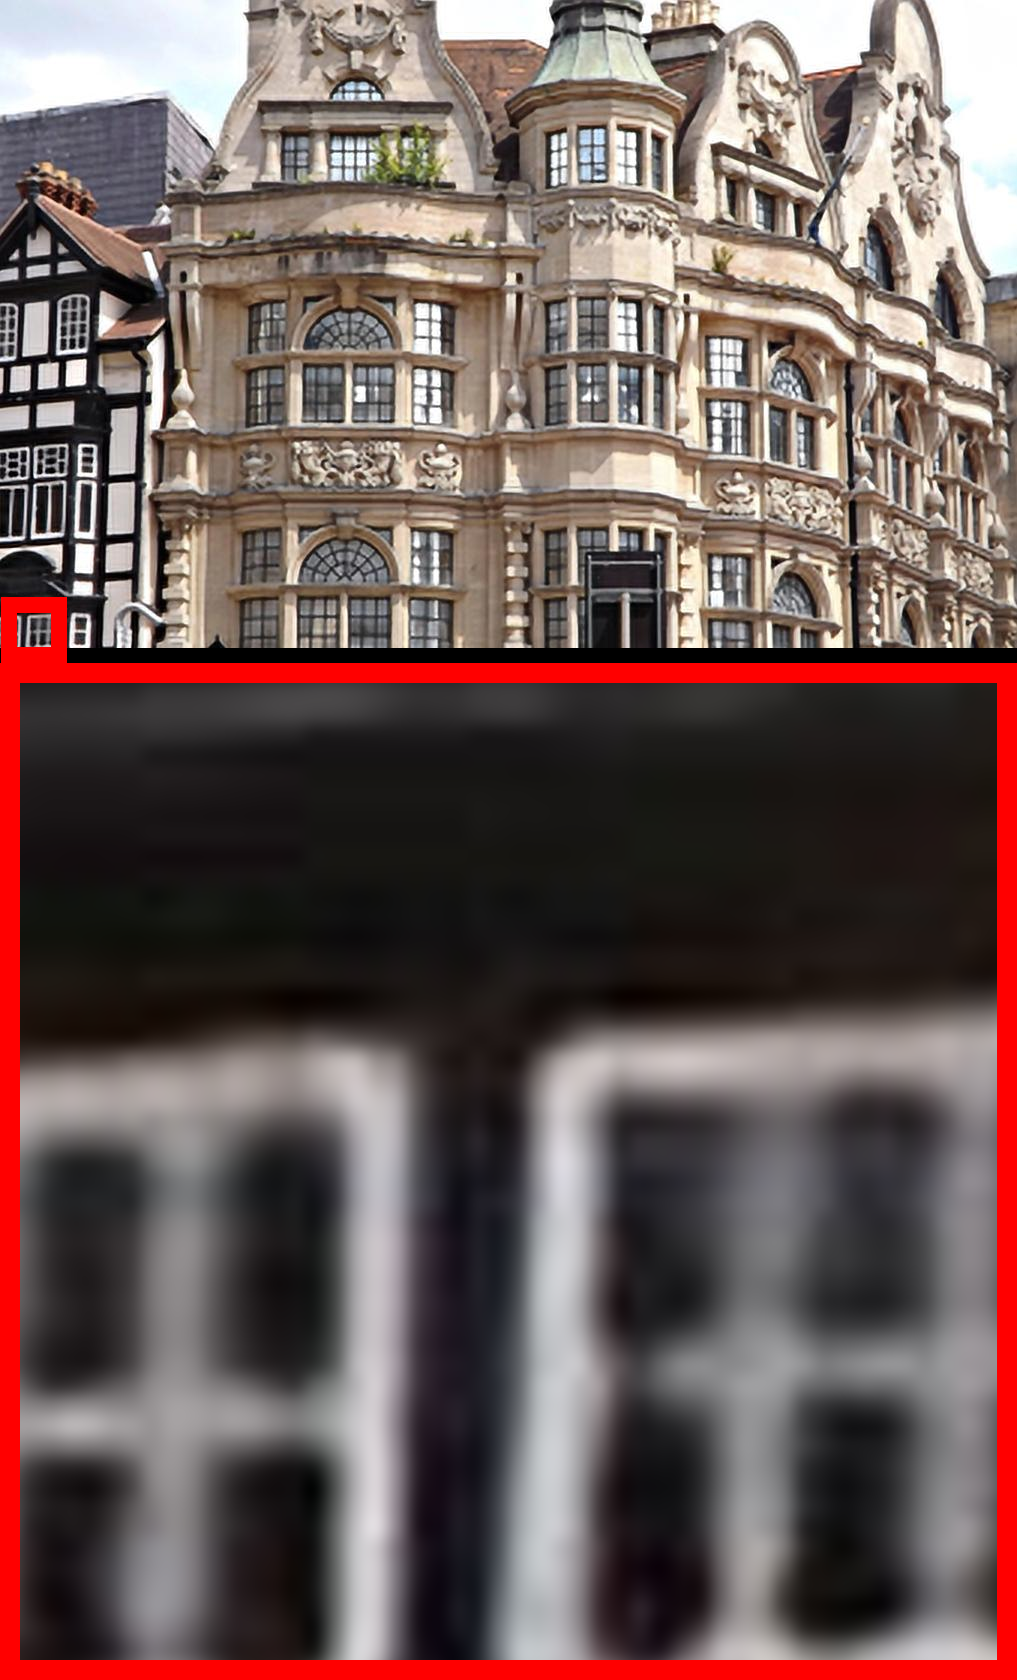
\includegraphics[width=0.23\textwidth]{img_053_7_w.png} &
\graphicspath{{figs/}}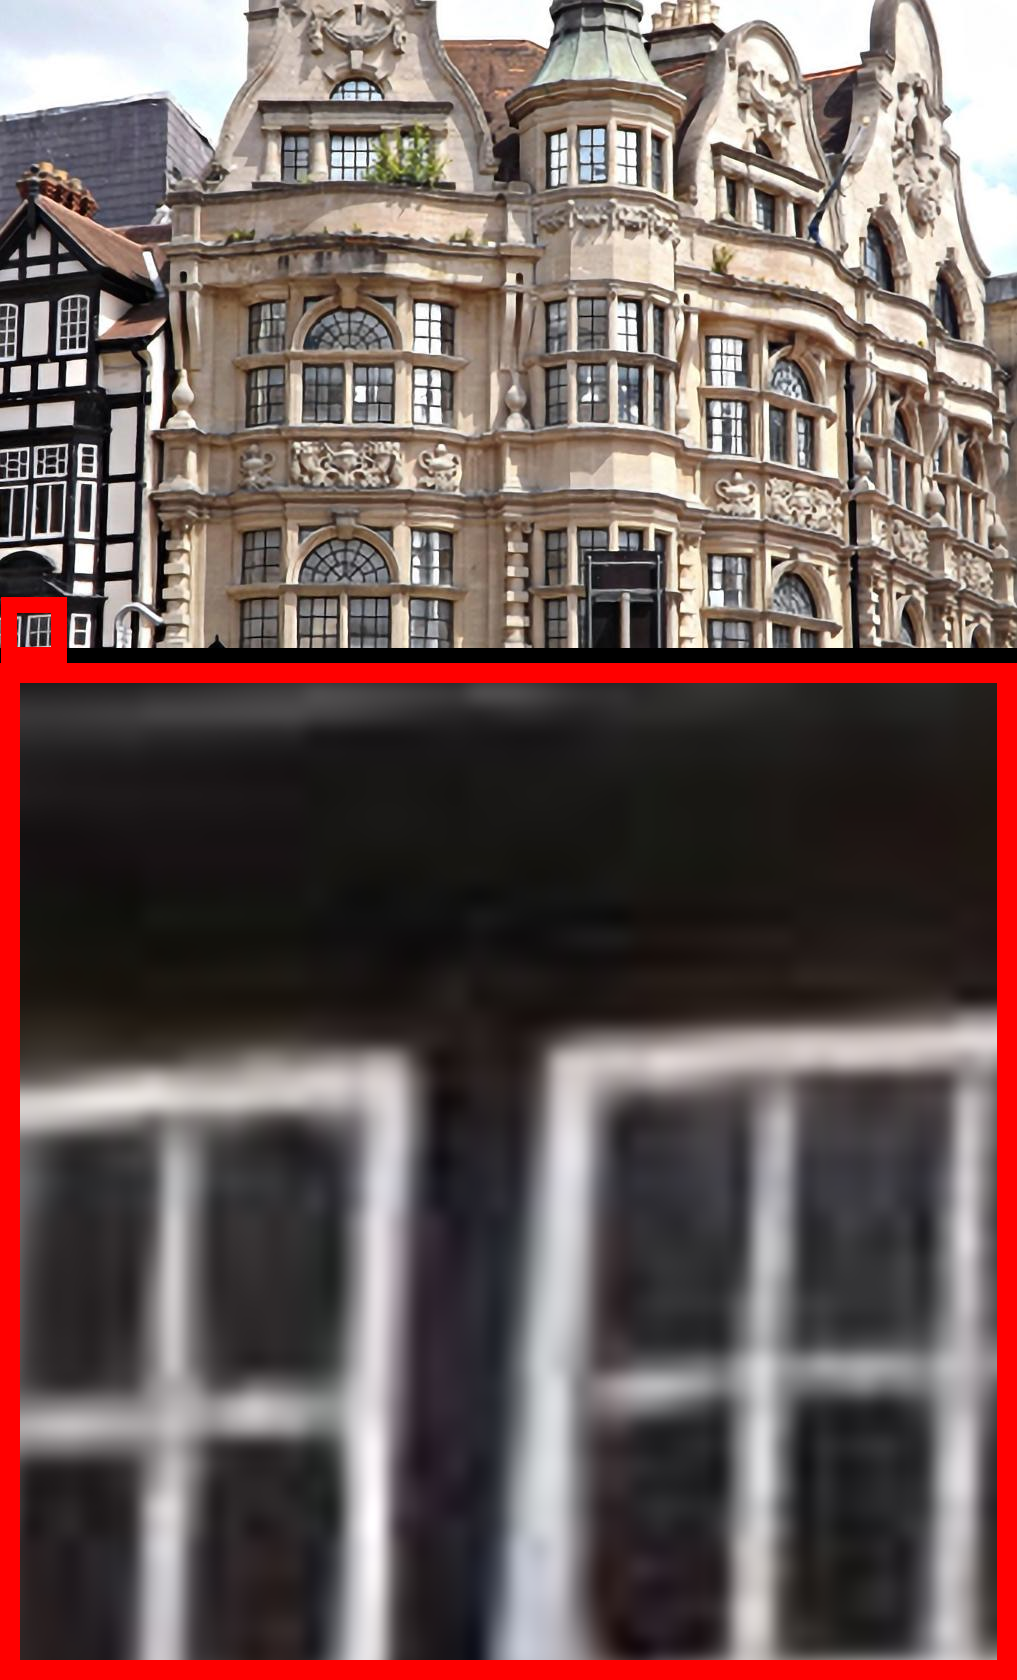
\includegraphics[width=0.23\textwidth]{img_053_9_w.png} 
\\
Original / PSNR (dB) &A+ / 22.31 &SRCNN / 22.34 &RCN (Ours) / 23.13 \\
\end{tabular}
\end{center}
\vspace{-.5cm}
\caption{Super-resolution results (Urban100) with scale factor $\times$3. Our result is visually pleasing.}\label{fig:c2}
\end{figure*}


\begin{figure*}
\begin{center}
\begin{tabular}{cccc}
\graphicspath{{figs/}}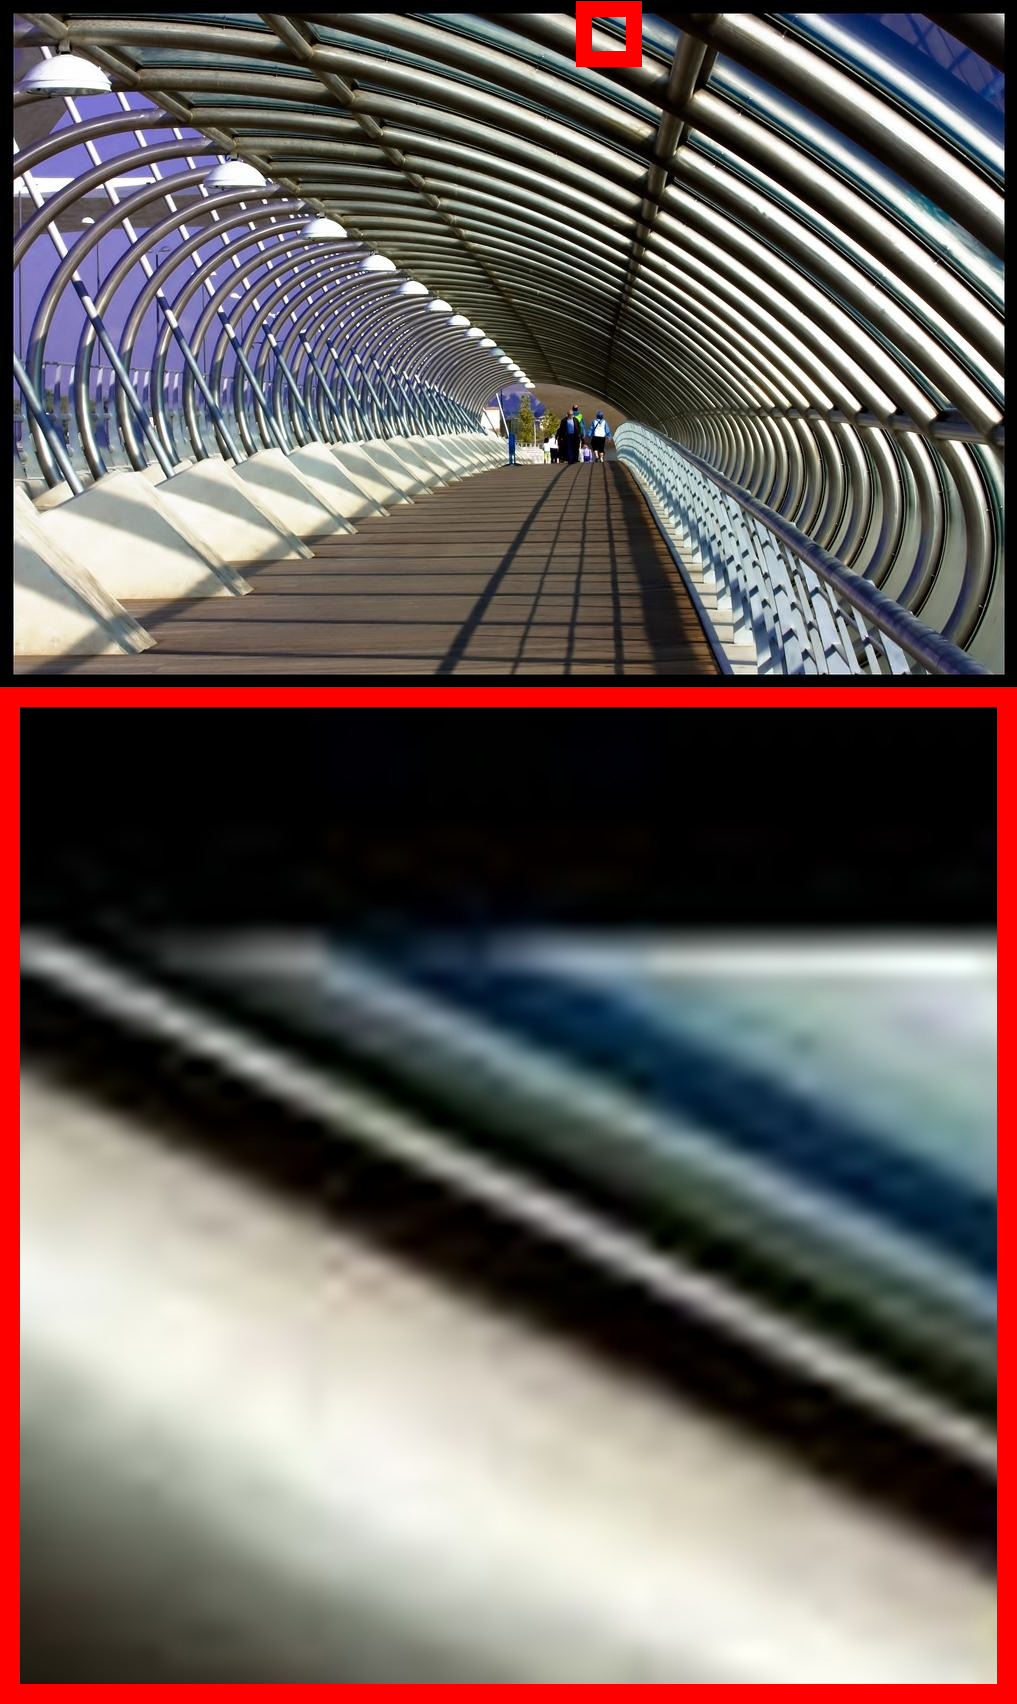
\includegraphics[width=0.23\textwidth]{img_058_1_w.png} &
\graphicspath{{figs/}}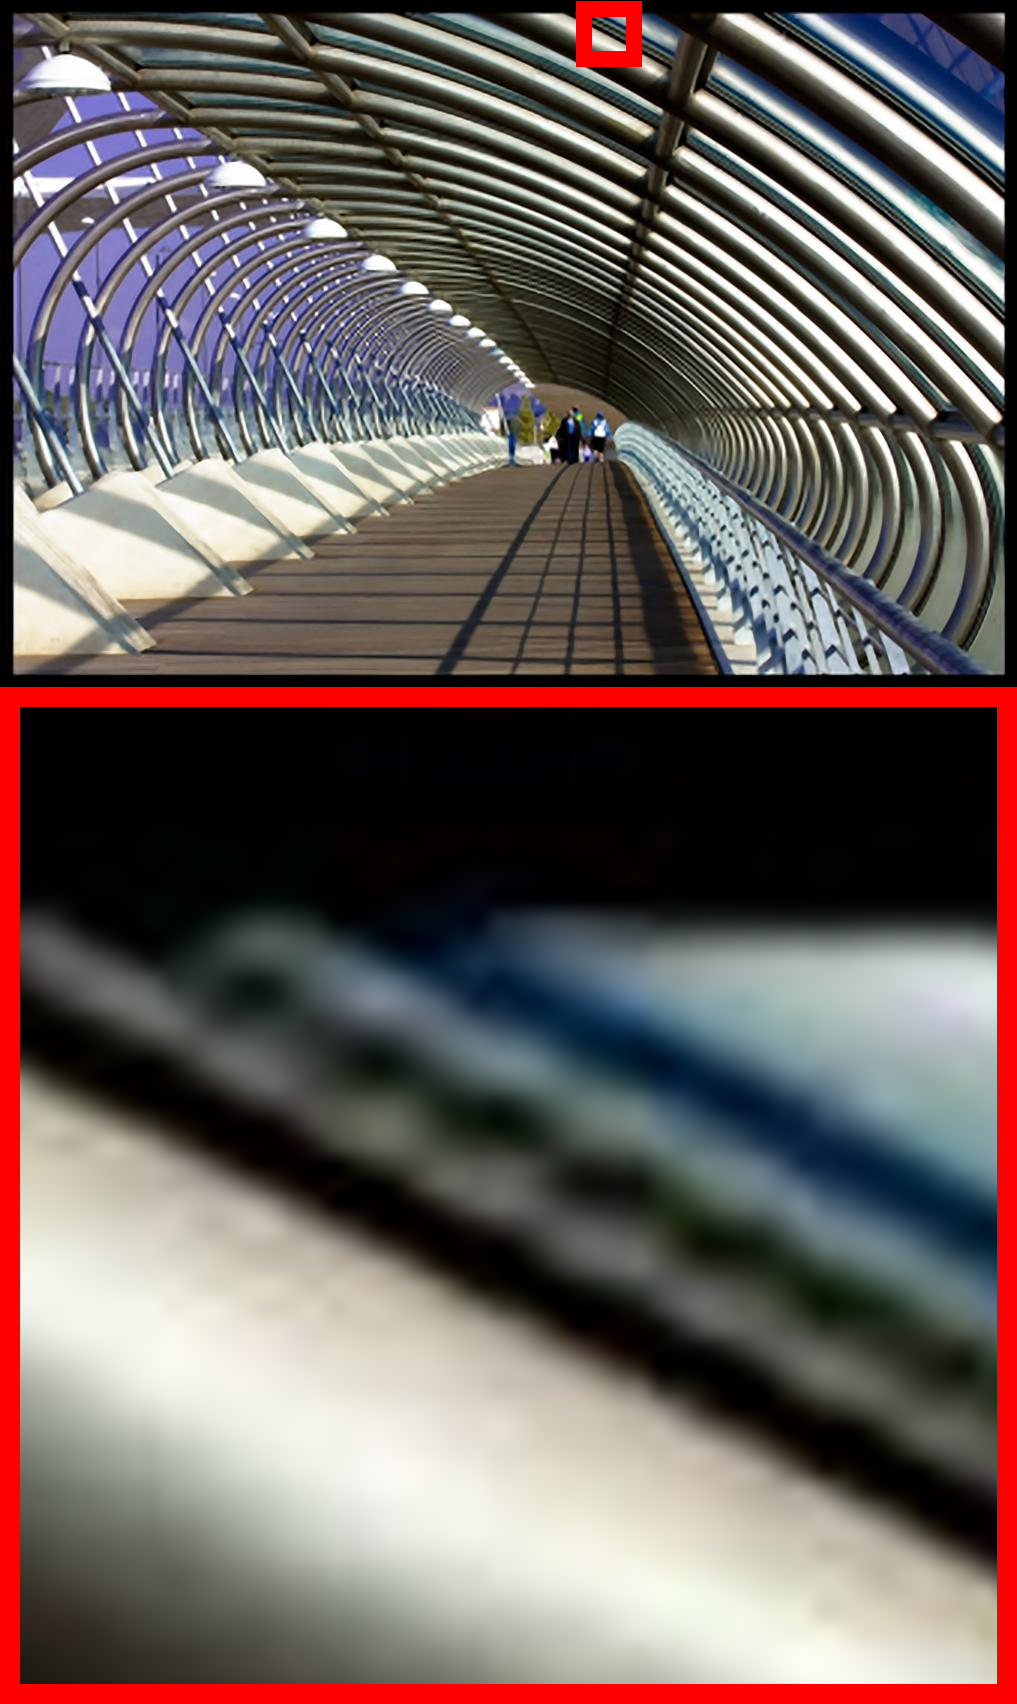
\includegraphics[width=0.23\textwidth]{img_058_6_w.png} &
\graphicspath{{figs/}}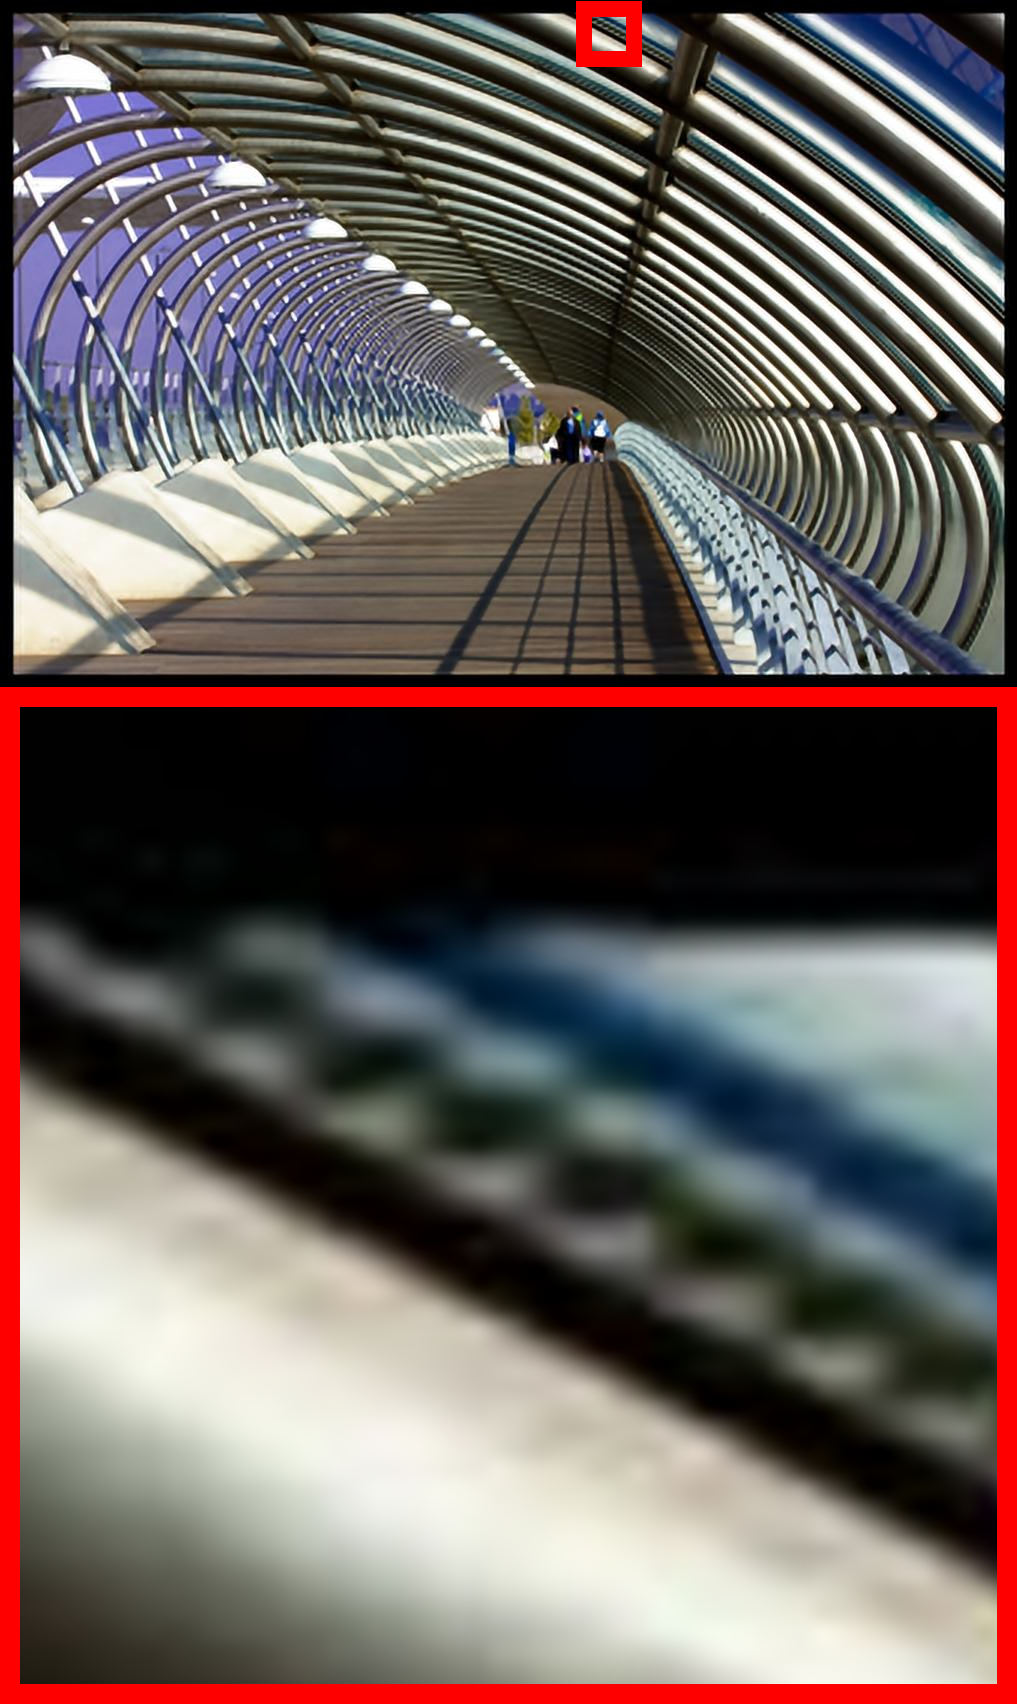
\includegraphics[width=0.23\textwidth]{img_058_7_w.png} &
\graphicspath{{figs/}}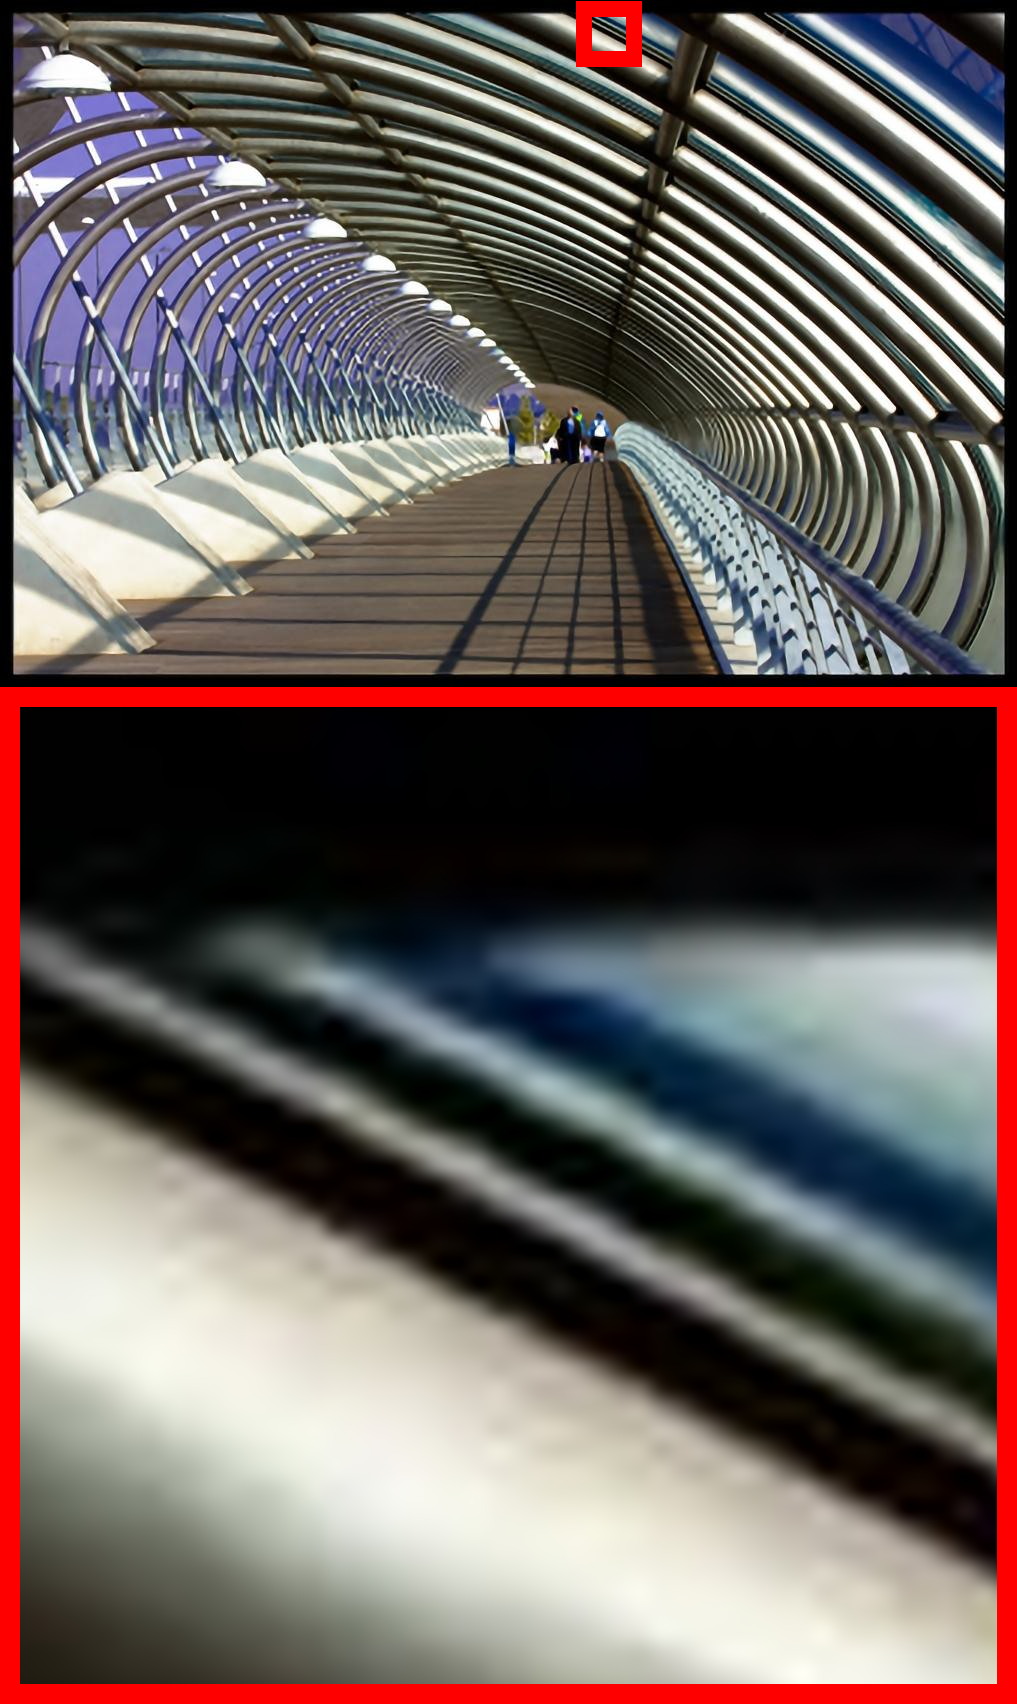
\includegraphics[width=0.23\textwidth]{img_058_9_w.png} 
\\
Original / PSNR (dB) &A+ / 25.87 &SRCNN / 25.76 &RCN (Ours) / 26.57 \\
\end{tabular}
\end{center}
\vspace{-.5cm}
\caption{Super-resolution results (Urban100) with scale factor $\times$3. Our result is visually pleasing.}\label{fig:c3}
\end{figure*}

\subsection{High Depths for Large Contexts}
In this section, we study the depth of a convolutional neural network (CNN) in the context of super-resolution. We first start with the definition of receptive field in a CNN. 

CNNs exploit spatially-local correlation by enforcing a local connectivity pattern between neurons of adjacent layers \cite{Bengio-et-al-2015-Book}. In other words, hidden units in layer $m$ take as input a subset of units in layer $m-1$. They form spatially contiguous receptive fields (Figure \ref{fig:receptive_field}).

Imagine that layer $m-1$ is the input image. In the figure, units in layer $m$ have receptive fields of 3$\times$3 in the input and are thus only connected to 9 adjacent neurons in the input layer. Units in layer $m+1$ have a similar connectivity with the layer below. We say that their receptive field with respect to the layer below is 3$\times$3, but their receptive field with respect to the input is larger (5$\times$5). Each unit is unresponsive to variations outside of its receptive field with respect to the input. The architecture thus ensures that the learned filters produce the strongest response to a spatially local input pattern.

However, as shown above, stacking many such layers leads to filters that become increasingly “global” (i.e. responsive to a larger region of pixel space). For example, the unit in hidden layer $m+1$ can encode a non-linear feature of 5$\times$5 (in terms of image pixel space).

In this work, we use small filters of the same size 3$\times$3 for all layers. For the first layer, its receptive field is of size 3$\times$3. For the next layers, the size of its receptive field increases by 2 in both height and width. For depth $M$ network, its receptive field has size $(2M+1)\times(2M+1)$. Its size is proportional to the depth.

In the task of SR, this corresponds to the amount of contextual information that can be exploited to infer high-frequency components. Large receptive field means the network can use more context from large image region to predict details of an image. As SR is an ill-posed inverse problem, collecting and analyzing more neighbor pixels give more clues. For example, if there are some image patterns entirely contained in a receptive field, it is plausible that this pattern is recognized and used to super-resolve the image. 

We now experimentally show that very deep networks significantly improve performance.  Since our layers are of the same type, we train and test networks of depth ranging from 5 to 20 (only counting weight layers excluding nonlinearity layers). 

In Figure \ref{fig:depth}, we show the results. In most cases, performance increases as depth increases. The exception is scale factor 2. As depth increases, performance on scale factors 3 and 4 improve rapidly. Since we use Euclidean loss, it tends to correct severe errors first, which are more prevalent in high scale factors. Different loss functions can be explored to balance the importance between scales and these are left as a future work. 

\begin{table*}
\footnotesize
\begin{center}
\begin{tabular}{ |c|c|c|c|c|c|c|c|c|c| }
\hline
\multirow{2}{*}{Dataset} & \multirow{2}{*}{Scale} & {Bicubic} & {A+} & {SRCNN} & {Huang et al.} & {RCN} & {RCN-291} & {RCN+} & {RCN-291+ (Ours)}\\ 

 &  & PSNR/Time & PSNR/Time & PSNR/Time & PSNR/Time & PSNR/Time & PSNR/Time & PSNR/Time & PSNR/Time\\ 
\hline
\hline
\multirow{3}{*}{Set5}
& $\times$2& 33.66 / - & 36.55 / 0.44& 36.66 / 2.12& -& 37.06 / 0.31& \color{blue} 37.38 / 0.15& 37.24 / 0.18& \color{red} 37.53 / 0.19\\
& $\times$3& 30.39 / - & 32.59 / 0.23& 32.75 / 2.13& -& 33.27 / 0.22& 33.42 / 0.15& \color{blue} 33.50 / 0.18& \color{red} 33.67 / 0.19\\
& $\times$4& 28.42 / - & 30.28 / 0.16& 30.49 / 2.21& -& 30.95 / 0.22& 31.09 / 0.15& \color{blue} 31.22 / 0.18& \color{red} 31.35 / 0.19\\
\hline
\hline
\multirow{3}{*}{Set14}
& $\times$2& 30.23 / - & 32.28 / 0.92& 32.45 / 3.79& -& 32.61 / 0.32& \color{blue} 32.84 / 0.21& 32.77 / 0.26& \color{red} 33.04 / 0.27\\
& $\times$3& 27.54 / - & 29.13 / 0.48& 29.30 / 3.78& -& 29.48 / 0.32& 29.63 / 0.21& \color{blue} 29.64 / 0.26& \color{red} 29.77 / 0.27\\
& $\times$4& 26.00 / - & 27.32 / 0.34& 27.50 / 3.80& -& 27.71 / 0.32& 27.85 / 0.21& \color{blue} 27.91 / 0.26& \color{red} 28.01 / 0.27\\
\hline
\hline
\multirow{3}{*}{Urban100}
& $\times$2& 26.61 / - & 28.57 / 3.15& 28.82 / 12.78& -& 29.22 / 0.76& \color{blue} 29.52 / 0.51& 29.41 / 0.67& \color{red} 29.76 / 0.68\\
& $\times$3& 24.36 / - & 25.82 / 1.68& 25.99 / 12.85& -& 26.35 / 0.76& 26.52 / 0.51& \color{blue} 26.53 / 0.67& \color{red} 26.76 / 0.68\\
& $\times$4& 23.07 / - & 24.22 / 1.17& 24.40 / 12.60& 24.55 / -& 24.62 / 0.77& 24.78 / 0.51& \color{blue} 24.82 / 0.67& \color{red} 24.99 / 0.68\\
\hline
\hline
\multirow{3}{*}{B100}
& $\times$2& 29.32 / - & 30.77 / 0.58& 30.89 / 2.43& 30.70 / -& 31.02 / 0.25& \color{blue} 31.21 / 0.17& 31.13 / 0.21& \color{red} 31.30 / 0.22\\
& $\times$3& 27.15 / - & 28.18 / 0.31& 28.28 / 2.48& 28.10 / -& 28.42 / 0.25& \color{blue} 28.55 / 0.17& 28.52 / 0.21& \color{red} 28.64 / 0.22\\
& $\times$4& 25.92 / - & 26.77 / 0.22& 26.84 / 2.39& 26.74 / -& 26.98 / 0.25& \color{blue} 27.10 / 0.17& 27.08 / 0.20& \color{red} 27.20 / 0.21\\
\hline
\end{tabular}
\end{center}
\caption{PSNR for scale factor $\times$2, $\times$3 and $\times$4 on datasets `Set5', `Set14', `Urban100', and `B100'. {\color{red} Red color} indicates the best performance and {\color{blue}blue color} indicates the second best one.} \label{table_all}
\end{table*}

\section{Experimental Results}
In this section, we evaluate the performance of our method on several datasets. We first describe datasets used for training and testing our method. Next, parameters necessary for training are given. 

After outlining our experimental setup, we compare our method with several state-of-the-art SISR methods. 

\subsection{Datasets for Training and Testing}
\textbf{Training dataset} For training, we use images proposed in Yang et al. \cite{yang2010image}, which is used by other learning-based methods \cite{Timofte,Timofte2013,zeyde2012single}. 

\textbf{Test dataset} For benchmark, we use four datasets. Datasets `Set5' \cite{bevilacqua2012} and `Set14' \cite{zeyde2012single} are often used for benchmark in other works \cite{Timofte,Timofte2013,Dong2014}. Dataset `Urban100', a dataset of urban images recently provided by Huang et al. \cite{Huang-CVPR-2015} is very interesting as it contains many challenging images failed by many of existing methods. Finally, dataset `B100', natural images in the Berkeley Segmentation Dataset, used in Timofte et al. \cite{Timofte} and Yang and Yang \cite{Yang2013} for benchmark, is also employed. 
\subsection{Training Parameters}
We provide parameters used to train our final model. We use a network of depth 20. Training uses batches of size 64. Momentum and weight decay parameters are set to 0.9 and $0.0001$, respectively. 

For weight initialization, we use the method described in He et al. \cite{he2015delving}. This is a theoretically sound procedure for networks utilizing rectified linear units (ReLu).

We train all experiments over 80 epochs (9960 iterations with batch size 64). Learning rate was initially set to 0.1 and then decreased by a factor of 10 every 20 epochs. In total, the learning rate was decreased 3 times, and the learning
is stopped after 80 epochs. Training takes roughly 4 hours on GPU Titan X. 

%\footnotetext{\textcolor{red}{PSNRs are slightly different from the original paper as they use different evaluation framework from Timofte et al. \cite{Timofte}}}

\subsection{Benchmark}
For benchmark, we follow the publicly available framework of Timofte et al. \cite{Timofte2013}. It enables the comparison of many state-of-the-art results with the same evaluation procedure.

The framework applies bicubic interpolation to color components of an image and sophisticated models to luminance components as in  other methods \cite{chang2004super}, \cite{glasner2009super}, \cite{zeyde2012single}. This is because human is much more sensitive to visually observe details in intensity than in color. 


This framework crops pixels near image boundary. For our method, this procedure is unnecessary as our network super-resolves an entire image. For fair comparison, however, we also crop pixels to the same amount.



\subsection{Comparisons with State-of-the-Art Methods}
We provide quantitative and qualitative comparisons. Compared methods are A+ \cite{Timofte}, SRCNN \cite{Dong2014} and Huang et al. \cite{Huang-CVPR-2015}.

In Table \ref{table_all}, we provide a summary of quantitative evaluation on several datasets. In addition to our model trained with 91 images, we provide three more models. A model trained with 291 images (91 + 200 natural images from Berkeley Segmentation Dataset \cite{Martin2001}).
We also provide RCN+ and RCN-291+, where transformed images (combination of flips and 90 deg. rotations) are also used for training. Our methods outperform all previous methods in these datasets. Moreover, our methods are very fast.

In Figures \ref{fig:c1}, \ref{fig:c2} and \ref{fig:c3} we compare our method with top-performing methods. In Figure \ref{fig:c1}, only our method perfectly reconstructs the line in the middle. Similarly, in Figures \ref{fig:c2} and \ref{fig:c3}, lines are clean and vivid in our method whereas they are severely blurred or distorted in other methods. As Huang et al. does not publicly provide $\times 3$ results we only compare with other two methods.

\section{Conclusion}
In this work, we have presented a single-model super-resolution method. Our method uses a very deep convolutional network modified for learning an residual (output minus input). We demonstrate three properties. First, we show our method works under various scales. Second, optimizing a residual-learning network converges rapidly toward a state-of-the-art solution. Third, very deep network operating on an large image region improves performance for large scale factors. We have demonstrated that our method outperforms the existing method by a large margin on benchmarked images. In the future, one can try a much deeper network in order to use full image-level information (receptive field larger than image). Residual-learning network is also readily applicable to other image restoration problems such as denoising and deblurring.

{\small
	\bibliographystyle{ieee}
	\bibliography{VDSR}
}
\end{document}
